\documentclass[11pt,a4paper]{article}

% ---------- packages ----------
\usepackage[utf8]{inputenc}
\usepackage[margin=1in]{geometry}
\usepackage{amsmath,amssymb,mathtools}
\usepackage{amsthm}
\usepackage{siunitx}
\usepackage{booktabs}
\usepackage{array}
\usepackage{longtable}
\usepackage{xcolor}
\usepackage{listings}
\usepackage{enumitem}
\usepackage[most]{tcolorbox}
\usepackage[expansion=false]{microtype}
\usepackage{parskip}
\usepackage{fancyhdr}
\usepackage{hyperref}
\usepackage{tikz}
\usetikzlibrary{positioning,arrows.meta,calc}
\usepackage{pgfplots}
\pgfplotsset{compat=1.18}
\usepackage{cleveref}

% ---------- colours ----------
\definecolor{kw}{HTML}{0B6FA4}
\definecolor{str}{HTML}{2E7D32}
\definecolor{cmt}{HTML}{777777}
\definecolor{seam}{HTML}{0B6FA4}
\definecolor{boxbg}{HTML}{F4F8FB}
\definecolor{rule}{HTML}{C9D6DF}

\hypersetup{colorlinks=true, linkcolor=kw, urlcolor=kw, citecolor=kw,
  pdftitle={Cavendish --- Gravitational Atom-Gradiometer Simulator Specification},
  pdfauthor={Malachy}}

% ---------- siunitx ----------
\sisetup{per-mode=symbol, separate-uncertainty=true}

% ---------- listings ----------
\lstdefinestyle{rs}{
  basicstyle=\footnotesize\ttfamily,
  keywordstyle=\color{kw}\bfseries,
  commentstyle=\color{cmt}\itshape,
  stringstyle=\color{str},
  numbers=left, numberstyle=\tiny\color{cmt}, numbersep=8pt,
  showstringspaces=false, breaklines=true, columns=fullflexible,
  keepspaces=true, frame=single, rulecolor=\color{rule}, framesep=6pt,
  backgroundcolor=\color{boxbg}, xleftmargin=14pt, aboveskip=10pt, belowskip=6pt,
  morekeywords={fn,let,mut,struct,trait,impl,for,in,if,else,match,return,pub,enum,
    Box,dyn,Vec,Self,Option,Some,None,Result,Ok,Err,f64,u32,usize,bool,as,where,
    type,const,move,async,await,use,mod,loop,while,break,continue}
}
\lstset{style=rs}

% ---------- theorem-like environments ----------
\newtheoremstyle{reqstyle}{8pt}{8pt}{\normalfont}{0pt}{\bfseries}{.}{ }%
  {\thmname{#1}\thmnumber{-#2}\thmnote{ \normalfont(\itshape#3\normalfont)}}
\theoremstyle{reqstyle}
\newtheorem{freq}{FR}
\newtheorem{nfreq}{NFR}

% contract / seam boxes
\newtcolorbox{seambox}[1]{colback=boxbg, colframe=seam, fonttitle=\bfseries,
  coltitle=white, title={#1}, boxrule=0.6pt, arc=2pt, left=6pt, right=6pt,
  top=4pt, bottom=4pt, breakable}

\newtcolorbox{contractbox}[1]{colback=white, colframe=rule, fonttitle=\bfseries,
  coltitle=black, title={#1}, boxrule=0.6pt, arc=1pt, left=6pt, right=6pt,
  top=4pt, bottom=4pt, breakable}

% ---------- math shorthands ----------
\newcommand{\rv}{\mathbf{r}}
\newcommand{\vv}{\mathbf{v}}
\newcommand{\xv}{\mathbf{x}}
\newcommand{\rhat}{\hat{\mathbf{r}}}
\newcommand{\grad}{\nabla}
\newcommand{\dd}{\,\mathrm{d}}
\newcommand{\half}{\tfrac{1}{2}}
\DeclareMathOperator{\tr}{tr}

% ---------- headers ----------
\pagestyle{fancy}
\fancyhf{}
\fancyhead[L]{\footnotesize\textsc{Cavendish}}
\fancyhead[R]{\footnotesize Simulator Specification}
\fancyfoot[C]{\thepage}
\renewcommand{\headrulewidth}{0.4pt}
\setlength{\emergencystretch}{2em}

% =====================================================================
\begin{document}

\begin{titlepage}
\centering
\vspace*{2.2cm}
{\Huge\bfseries Cavendish\par}
\vspace{0.5cm}
{\Large A Gravitational Atom-Gradiometer Simulator\par}
\vspace{0.3cm}
{\large Engineering \& Physics Specification\par}
\vspace{1.6cm}
{\large Draft v0.5\par}
\vspace{0.4cm}
{\normalsize\today\par}
\vspace{2.4cm}
\begin{minipage}{0.82\textwidth}
\small\itshape
A Rust library that simulates the differential phase an atom-interferometer gradiometer
array (AION-10 geometry) reads from moving external masses, and emits the full
per-measurement state --- source kinematics, mass distribution, gravitational field, and
the noisy multi-detector signal --- as a live stream of tensors. Its purpose is to be the
data engine for \emph{Gradar} (passive gradiometric tracking): a learned tracker that recovers the
time-resolved tracks of moving masses (gravity-gradient noise) from the joint signal across
a spatially separated array, with coherent ultralight dark matter sitting in the same data
as the common-mode channel the tracker rejects.
\end{minipage}
\vspace{2.4cm}

{\normalsize Malachy\par}
\vfill
{\footnotesize The forward model and validation targets are taken from G.\ Parish,
\emph{Charting New Frontiers in Dark Matter Detection using Atom Interferometry}
(KCL/RAL upgrade report, 2026), and his reference implementation, which together serve as
the numerical oracle.\par}
\end{titlepage}

\tableofcontents
\newpage

\section{Introduction}

\subsection{Purpose}
Cavendish simulates the gravitational \emph{gravity-gradient noise} (GGN) signal that
moving external masses induce in an array of atom-interferometer gradiometers, and produces
the complete physical state of each scenario as machine-learning--ready tensors. Its purpose
is to be the data engine for \emph{Gradar}: a learned tracker that solves the
inverse problem of recovering the \emph{time-resolved tracks} of the moving sources --- their
positions over time, hence velocities and trajectories, and how many there are --- from the
joint multi-detector signal. This is passive (no emission; the masses' own static fields are
read as they move), and the spatial separation of the array is what makes position
identifiable (\Cref{sec:array,sec:radar}).

The instrument modelled is a Cavendish-class device. In a laboratory G-measurement the
source mass is known and one solves the differential phase for $G$; Cavendish runs the
identical forward map inverted --- $G$ is held fixed and the source is the unknown. The
gradiometer geometry, atom species and timing follow the AION-10 experiment.

\subsection{Context}
The forward model, instrument parameters and validation targets are taken from
G.~Parish's upgrade report~\cite{parish2026} and his reference code, which characterise GGN
from oscillating masses for AION-10, extending the constant-velocity treatment of Carlton \&
McCabe~\cite{carlton2023}. That work reframes the problem the simulator serves: its
scientific target is \emph{ultralight dark matter} (ULDM), a coherent phase oscillation at
$f_\phi \approx \SI{0.1}{\hertz}$ (\Cref{sec:uldm}); the moving masses (lifts, oscillating
plant) are the GGN \emph{background} to be removed. So Cavendish's moving-mass forward model
\emph{is} the GGN model, and the two live in the same data split by spatial coherence: a
local mass is differential across the array (the Gradar target), a coherent ULDM field is
common-mode (the same data, the channel the tracker rejects).

The reference code is adopted as the numerical \emph{oracle}: Cavendish must reproduce it to
$\geq 99\%$ on the point-mass cases, converge to its extended-body integrals, and recover the
ULDM line through its analysis pipeline (\Cref{sec:tests}). The report itself names
``machine-learning approaches trained on the simulation outputs developed here'' as the next
step~\cite{parish2026}; Cavendish is that data engine.

\subsection{Design philosophy}
Three principles fix the architecture.

\begin{enumerate}[leftmargin=*]
\item \textbf{One currency: $\rho(\xv,t)$.} The gravity kernel needs only the mass-density
field as a function of space and time, discretised to a cloud of mass elements per tick.
Every source --- a rigid body, a walking person, a sloshing fluid, a vibrating floor --- is
just a different way of producing $\rho(\xv,t)$. The kernel, the forward model and the data
contract never change as sources are added.

\item \textbf{Live generation.} The library runs as a data source, not a precomputed
dataset: a training loop requests scenarios and the library generates and streams them on
demand. Disk is an optional cache, not the path.

\item \textbf{The engine dumps the entire state; the task lives downstream.} A single typed
bundle (\Cref{tab:bundle}) is the only coupling between the engine and anything downstream, and
it is \emph{complete}: the simulator emits the full per-measurement record --- source kinematics,
mass distribution, field, the \emph{multi-channel} signal (one differential-phase series per
detector in the array, \Cref{sec:array}), the time-resolved source tracks and their count, the
contamination mask, derived spectra --- all as ground truth at generation time. Generating ML
datasets at scale is a primary intended use, and the engine is built for it (batched, reproducible
from a seed, tensor-native); but it serves that use by emitting the \emph{whole} record and letting
the consumer decide what is input, label, target, or context. The supervised, self-supervised, and
analysis structure lives entirely downstream --- which is precisely what keeps the dump total, and
every downstream use (a tracker, a world-model, a Cram\'er--Rao study, one not yet imagined)
possible. A model later produces a prediction against the bundle; a viewer renders either.
\end{enumerate}

\section{Scope}
\label{sec:scope}

\subsection{Version 1 (this specification)}
\begin{itemize}[leftmargin=*,nosep]
\item \textbf{Source:} rigid bodies only --- arbitrary mesh $\to$ voxel cloud, with analytic
primitives as the oracle; a library of prescribed/physical trajectories (static, linear
pass, 1D/2D/3D oscillation, circular, lift, pendulum, spin, rocking, and free rotation --- the
Euler top); composition of independent sources,
including \emph{multiple simultaneous targets} (the multi-target Gradar case).
\item \textbf{Instrument:} an \emph{array} of vertical gradiometers at configurable ground
placements (\Cref{sec:array}); $N{=}1$ recovers a single gradiometer.
\item \textbf{Forward model:} the propagation-phase double-difference integral
(\Cref{sec:forward}), evaluated per detector along the four parabolic arm trajectories.
\item \textbf{ULDM:} the closed-form coherent dark-matter phase (\Cref{sec:uldm}) as an
additive common-mode signal, the separation target the Gradar tracker rejects.
\item \textbf{Gravity:} direct element sum near-field; multipole expansion far-field;
swappable discretisation element (point default; sphere, cube).
\item \textbf{Measurement schedule:} a realistic, seedable cadence model
(\Cref{sec:schedule}) --- cycle jitter, shot failures, scheduled (e.g.\ nighttime) gaps, and
Poisson transient (lift) events with contamination tagging --- yielding non-uniformly sampled
series; a uniform default is the degenerate case.
\item \textbf{Noise:} a pluggable, seedable stack (shot noise, vibration residual); may
ship empty and grow, since the forward model validates noiseless.
\item \textbf{Compute:} the parallel field-evaluation hot path on GPU, the sequential glue on
CPU (\Cref{sec:compute}); CPU-only is a valid fallback for the reference path.
\item \textbf{Interfaces:} a Python SDK (\texttt{run}, \texttt{stream}) and thin CLI; a
native \texttt{egui}/\texttt{wgpu} debug viewer.
\item \textbf{Output:} the state bundle as torch-ready tensors, live --- the multi-detector
signal, the time-resolved track labels, the Lomb--Scargle periodogram; optional frozen cache.
\end{itemize}

\subsection{Deferred (seams kept, not built)}
Non-rigid source dynamics (articulated bodies, deforming bodies, compressible and
incompressible fluids), structural vibration, airflow/convection (\Cref{sec:parked}); the
learned Gradar tracker itself, which \emph{consumes} the stream (\Cref{sec:radar}); and the
arbitrary-orientation interferometer (v1 arrays are horizontally separated \emph{vertical}
gradiometers). The Fisher-information / Cram\'er--Rao floor on what the array can identify is
in scope as an analysis output (\Cref{sec:radar}), enabled by the differentiable forward
model (\Cref{nfr:diff}).

\section{System Architecture}
\label{sec:arch}

\subsection{Crate and module map}
Dependency flows one way out of \texttt{sim-core}. The SDK is the primary consumer, the
viewer secondary: two Rust crates and one Python package.

\begin{lstlisting}
cavendish/
  crates/                 # the flat workspace; sim-core (the engine) = every crate but sdk/viewer
    math/                 # L0: vectors, quaternions, Isometry3, the Scalar trait (autodiff seam)
    config/               # L0: the one typed config schema (Prior, FieldSet)
    gravity/              # L1: Cloud, potential/field/gradient-tensor; C->I/Q reduction; FieldContribution
    reference/            # L1: independent oracle -- George's cases by direct quadrature (math only)
    shape/                # L2: geometry -> mass: primitives + voxeliser (Solid seam); mesh import (M10)
    source/               # L2: SourceDynamics; Trajectory library; rotation integrator; bodies via shape
    instrument/           # L2: detector array: gradiometer geometry, placements, arms; PhaseModel
    uldm/                 # L2: closed-form coherent dark-matter phase (common-mode signal)
    noise/                # L2: NoiseSource stack + atmospheric-GGN FieldContribution adaptor
    compute/              # L2: CPU reference + GPU (wgpu) field-evaluation backend
    scenario/             # L3: Scenario assembly + Prior/sampler + measurement Schedule
    state/                # L3: StateBundle (multi-detector signal + ground-truth tracks) + FieldSet
    generate/             # L4: per-scenario evaluation + batch (GPU dispatch / rayon)
    analysis/             # L5: Cramer-Rao / Fisher information via the Dual forward model
    sdk/                  # consumer: maturin/PyO3 package -- run()/stream() + CLI entry
    viewer/               # consumer: eframe/egui + wgpu (one-way dep on the engine)
  docs/
\end{lstlisting}

\subsection{The seams}
Four traits are the flex points; everything else is composition over them. Keeping these
clean is what lets the deferred features land as backends without touching the core.

\begin{seambox}{The four load-bearing traits}
\textbf{\texttt{GravitySource}} --- produces $V$, $\mathbf g$, $\Gamma$ at a world point.
Implemented by discretisation \emph{elements}, by the \emph{cloud} (element sum +
multipole far-field), and by analytic \emph{oracle} primitives.

\textbf{\texttt{SourceDynamics}} --- the mass configuration as a continuous function of
time, \texttt{cloud\_at(t)}. \texttt{Rigid} specialises it as pose~$\otimes$~body-cloud.

\textbf{\texttt{PhaseModel}} --- turns source $+$ instrument into the differential phase at
one measurement time. v1: the propagation integral.

\textbf{\texttt{NoiseSource}} --- one additive, seedable contribution to the signal; the
stack is a \texttt{Vec}.
\end{seambox}

\subsection{Generation modes}
Prescribed sources (\Cref{sec:parked}) run live inside \texttt{DataLoader} workers ---
cheap, stateless per tick, embarrassingly parallel. Solver-driven sources are too slow for
training-rate generation and integrate instead via \emph{cache-and-replay}: solve a modest
library of $\rho(\xv,t)$ fields offline, then place, scale and superpose them live as cheap
sources. This is the single point at which the live-generation model bends, and it bends by
design.

\subsection{Compute: the CPU/GPU split}
\label{sec:compute}
The cut between GPU and CPU is not chosen but read off the dependency structure of the
forward map: \textbf{the parallel arithmetic and its reductions run on the GPU; the
sequential glue, one-time setup and I/O stay on the CPU}. With voxel clouds at
$N\sim 10^5$--$10^7$ for extended bodies, the per-measurement field evaluation is the
expensive part and is the whole reason for the GPU --- a CPU-only path remains valid as the
reference but is too slow for training-rate generation.

\textbf{GPU --- the field-evaluation outer product.} Almost every axis is independent:
scenarios, measurements, detectors, interferometers, arms, and the within-flight
\texttt{fine\_dt} integrand samples are mutually independent; the only joins are two
\emph{reductions} (the sum over $N$ voxels for $V$ at a point, and the quadrature over the
flight for an arm's phase), which a GPU does well. The GPU therefore owns: source-pose and
atom-arm evaluation (closed-form, inline); the potential / gradient-tensor sum over the cloud
at every field point (the near-field $N$-body reduction); the multipole far-field branch; the
flight-integral quadrature; the differential-phase and gradiometer double-difference; and
noise injection via a counter-based RNG (philox/threefry), whose draw at each index is
parallel rather than sequential.

\textbf{CPU --- setup, control flow, I/O.} Voxelisation and the multipole reduction run
\emph{once per template at load} --- structurally parallel but amortised over millions of
scenarios, so there is no reason to ship them to the GPU; this is the only compute ever
legitimately on the CPU. Scenario sampling (discrete and branchy), kernel launch and
batching, and serialisation / the tensor handoff are the rest.

\textbf{The one sequential axis, kept on the GPU.} ODE-derived motion (the pendulum and free
rotation, \Cref{nfr:symplectic}) is sequential \emph{in time} --- which says CPU --- but independent
\emph{across scenarios}, and the poses it produces are consumed immediately by the field
evaluation. The deciding factor is locality, not parallelism: shipping CPU-integrated poses
would mean uploading source poses at \texttt{fine\_dt} resolution (the source moves
appreciably \emph{during} the \SI{1.46}{\second} flight), $\sim(\text{measurements}\times 146)$
poses per scenario --- gigabytes per batch. So the ODE is integrated on the GPU, one thread
per scenario, producing poses where they are consumed. The general rule across the bus:
\textbf{upload parameters, not poses} --- tiny trajectory-parameter sets and RNG keys go up,
poses are evaluated inline, the fat intermediate never comes back.

\begin{seambox}{Boundary contract}
\textbf{CPU $\to$ GPU:} the static body cloud, once per template; per-scenario trajectory
parameters $+$ RNG keys (tiny); instrument and array placements.\quad
\textbf{GPU $\to$ CPU:} the per-detector signal $\Delta\Phi_\ell$ and the per-measurement
state for the bundle.
\end{seambox}

No raw Vulkan: the native side uses \texttt{wgpu} compute (it already backs the viewer, sits
on Vulkan / Metal / DX12 anyway, and reuses the same device and WGSL shaders); the heavy
research-numerics path is vectorised in CUDA via the framework for zero-copy and autodiff. On
the \texttt{wgpu} path WGSL has no $f64$ and gravity differentials are tiny, so the kernel is
written \emph{differential-first} --- the gradient tensor / $\Gamma_{zz}L$ evaluated directly,
never two large absolute phases subtracted (\Cref{nfr:cond}) --- keeping $f32$ safely above the
mrad shot-noise floor. The multi-detector array adds one dimension to the outer product
(scenario $\times$ detector $\times$ timestep $\times$ field point): the same kernel, more
field points.

\subsection{The two representations}
\label{sec:tworep}
The one architectural decision that is genuinely expensive to change later --- and therefore
the one to fix now --- is the boundary between what the gravity kernel consumes and what each
source backend evolves. Two voxel representations exist, and they must stay separate.

\begin{itemize}[leftmargin=*,nosep]
\item \textbf{The gravity input} (what the kernel consumes) is the \texttt{Cloud}: elements of
$(\text{position},\text{mass})$ and at most an element-shape tag, nothing else. This is the
universal currency; it stays minimal forever, and the kernel never learns about material,
temperature, velocity, pressure or phase.
\item \textbf{The solver's own state} (what each backend evolves) is where material type,
temperature, velocity, pressure and compressibility live --- a convection solver carries a
temperature/velocity/density grid; a rigid body carries a pose; a vibration solver carries
modal amplitudes. Each backend holds whatever rich per-cell state its physics needs and
\emph{emits} a minimal \texttt{Cloud} through \texttt{cloud\_at(t)}.
\end{itemize}

Material phases --- \texttt{solid} and the compressible / incompressible fluid types --- are
therefore the \emph{solver's} cell types, not new fields on the gravity voxel. A single
universal voxel carrying $\{\text{mass},\text{material},\text{temperature},\dots\}$ would make
the kernel depend on the union of every physical property, so adding any new physics would
touch the core --- destroying the ``$\rho$ is the only currency'' decoupling the architecture
rests on (\Cref{fig:chokepoint}). Everything behind the cloud --- the fluid solver, the
temperature field, the skinning --- can land years later without touching the core, provided
this boundary is kept clean now.

\begin{figure}[h]
\centering
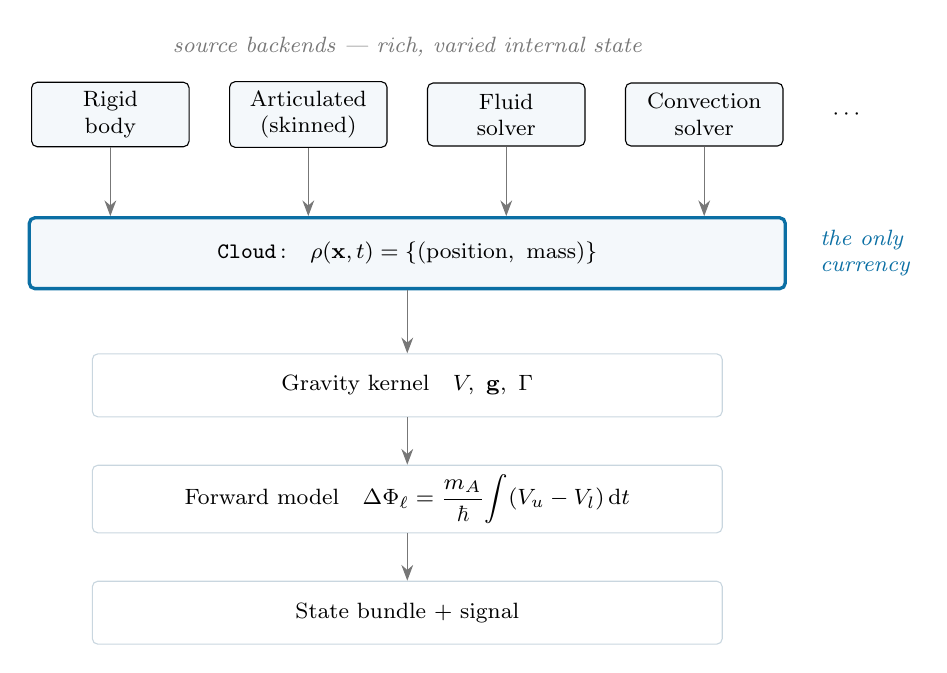
\begin{tikzpicture}[
  font=\footnotesize,
  src/.style={draw, rounded corners=2pt, fill=boxbg, minimum width=20mm, minimum height=8mm, align=center},
  hub/.style={draw=seam, very thick, rounded corners=2pt, fill=boxbg, minimum height=9mm, align=center},
  proc/.style={draw=rule, rounded corners=2pt, minimum height=8mm, align=center},
  ar/.style={-{Stealth[length=2mm]}, draw=cmt}
]
\node[src] (s1) {Rigid\\body};
\node[src, right=5mm of s1] (s2) {Articulated\\(skinned)};
\node[src, right=5mm of s2] (s3) {Fluid\\solver};
\node[src, right=5mm of s3] (s4) {Convection\\solver};
\node[right=5mm of s4] (sd) {$\cdots$};
\node[text=cmt, above=2mm of $(s1.north)!0.5!(s4.north)$] {\itshape source backends --- rich, varied internal state};

\node[hub, minimum width=96mm] (hub) at ($(s1.south)!0.5!(s4.south) - (0,1.35)$)
  {\textbf{\texttt{Cloud}}\,:\quad $\rho(\xv,t)=\{(\text{position},\ \text{mass})\}$};
\node[text=seam, right=3mm of hub.east, align=left] {\itshape the only\\\itshape currency};

\node[proc, below=8mm of hub, minimum width=80mm] (k) {Gravity kernel\quad $V,\ \mathbf g,\ \Gamma$};
\node[proc, below=6mm of k, minimum width=80mm] (f)
  {Forward model\quad $\Delta\Phi_\ell=\dfrac{m_A}{\hbar}\!\displaystyle\int(V_u-V_l)\dd t$};
\node[proc, below=6mm of f, minimum width=80mm] (o) {State bundle $+$ signal};

\draw[ar] (s1.south) -- (s1.south |- hub.north);
\draw[ar] (s2.south) -- (s2.south |- hub.north);
\draw[ar] (s3.south) -- (s3.south |- hub.north);
\draw[ar] (s4.south) -- (s4.south |- hub.north);
\draw[ar] (hub) -- (k);
\draw[ar] (k) -- (f);
\draw[ar] (f) -- (o);
\end{tikzpicture}
\caption{The minimal-cloud chokepoint. Every source backend, whatever its internal state,
emits the same minimal $\rho(\xv,t)$ cloud; the kernel and forward model see only that. New
physics is added as a new backend above the line, never as a change below it.}
\label{fig:chokepoint}
\end{figure}

\subsection{Conventions}
\label{sec:conventions}
The choices that, left implicit, surface later as a silent mismatch against George's code or
the asset importer --- fixed here by fiat, which is far cheaper than debugging a wrong frame.
\begin{itemize}[leftmargin=*,nosep]
\item \textbf{Frame and units.} World axes are right-handed with $z$ vertical (the tower
axis); gravity acts along $-z$. Lengths in metres, time in seconds, mass in kilograms --- SI
throughout, with no internal scaling.
\item \textbf{Orientation.} Quaternions are stored scalar-first ($w,x,y,z$) in the state
bundle; an imported glTF asset (scalar-last, $x,y,z,w$) is converted at the import boundary,
the only place the two conventions meet.
\item \textbf{Units in types.} Physical quantities use newtype wrappers
(\texttt{Metres(f64)}, \texttt{Seconds(f64)}, \texttt{Radians(f64)}) so the compiler refuses
to add a length to a time --- the cheapest defence against the unit bug.
\item \textbf{Pose ordering.} The per-tick pose is $(\text{position}_3,
\text{quaternion}_4)$ and the twist $(\text{linear}_3, \text{angular}_3)$, in that order,
matching \Cref{tab:bundle}.
\end{itemize}

\section{Physics and Mathematical Model}
\label{sec:physics}

This section states the physics Cavendish implements. Equation numbers in parentheses
refer to the source report~\cite{parish2026}; the model adopted here is the full
propagation-phase integral, not the uniform-field shortcut.

\subsection{The atom gradiometer}
The instrument is two Mach--Zehnder atom interferometers stacked vertically and
interrogated by common lasers (a gradiometer). Each interferometer splits a cloud of
ultracold $^{87}$Sr atoms with a $\tfrac{\pi}{2}$--$\pi$--$\tfrac{\pi}{2}$ pulse sequence;
the relative phase $\Delta\phi$ accumulated between the two arms sets the output port
populations,
\begin{equation}
P_{|g\rangle} = \cos^2\!\Big(\tfrac{1}{2}\Delta\phi\Big),
\qquad
P_{|e\rangle} = \sin^2\!\Big(\tfrac{1}{2}\Delta\phi\Big).
\end{equation}
The two interferometers, launched $\Delta r = \SI{5}{\metre}$ apart in a \SI{10}{\metre}
tower, are sensitive to the \emph{difference} in local gravity between them.

\begin{figure}[h]
\centering
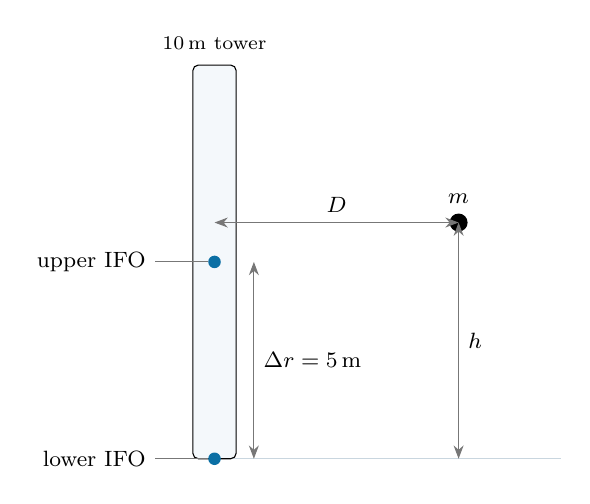
\begin{tikzpicture}[x=0.5cm,y=0.5cm,font=\footnotesize,
   dim/.style={<->,>=Stealth,draw=cmt},
   cloud/.style={circle,fill=seam,inner sep=1.6pt}]
\draw[draw=rule] (0,0) -- (8.8,0);
\draw[rounded corners=2pt,fill=boxbg,draw=black] (-0.55,0) rectangle (0.55,10);
\node[anchor=south,font=\scriptsize] at (0,10.15) {10\,m tower};
\node[cloud] (lo) at (0,0) {};
\node[cloud] (up) at (0,5) {};
\node[anchor=east] (ulab) at (-1.5,5) {upper IFO};
\node[anchor=east] (llab) at (-1.5,0) {lower IFO};
\draw[draw=cmt,thin] (ulab.east) -- (up);
\draw[draw=cmt,thin] (llab.east) -- (lo);
\draw[dim] (1.0,0) -- (1.0,5) node[midway,right]{$\Delta r=5$\,m};
\node[circle,fill=black,inner sep=2.3pt,label=above:{$m$}] (mass) at (6.2,6) {};
\draw[dim] (0,6) -- (6.2,6) node[pos=0.5,above]{$D$};
\draw[dim] (6.2,0) -- (6.2,6) node[midway,right]{$h$};
\end{tikzpicture}
\caption{Gradiometer geometry. Two $^{87}$Sr clouds, launched $\Delta r=\SI{5}{\metre}$ apart
in a \SI{10}{\metre} tower, interrogate vertically; an external mass at horizontal distance
$D$ and height $h$ perturbs the local potential, and the gradiometer reads the
\emph{difference} in its pull between the two interferometers.}
\label{fig:geometry}
\end{figure}

\subsection{The gradiometer array and the two channels}
\label{sec:array}
A single gradiometer cannot separate a coherent global oscillation from a local gravitational
transient at the same frequency; an array of them can, because the two have opposite spatial
signatures. The v1 array is several vertical gradiometers (each a tower as above) at distinct
ground positions $(x,y)$ --- the AION-network geometry; arbitrary orientation is deferred.

\textbf{Common-mode vs differential.} A ULDM field (\Cref{sec:uldm}) is spatially coherent
over its de Broglie length, which for a \SI{4e-16}{\electronvolt} scalar is of order an
astronomical unit --- vastly larger than any terrestrial array --- so every detector reads the
\emph{same} phase, in step: it is \emph{common-mode}. A local moving mass is a near-field
effect that falls off with distance and looks different metres away: it is \emph{differential}.
Hence \textbf{common-mode across the array $\to$ ULDM}, \textbf{differential across the array
$\to$ local GGN}. This is the discriminant a single device lacks, and it is what makes the
array the substrate for both detecting dark matter and tracking the masses that obscure it.

\textbf{Localisation.} The same separation gives source position. Differential amplitude
across detectors triangulates distance --- and because source mass is common-mode (it scales
every detector equally) while position is differential (it changes the ratios), the array
\emph{breaks the mass--distance degeneracy} a single gradiometer cannot. Relative timing of
closest approach and the differing tensor bearing at each detector add direction. This is
gravitational triangulation, the principle of a gravitational-wave or seismic network. Its
precision scales as (array baseline\,/\,source distance)\,$\times$\,SNR, quantified by the
Cram\'er--Rao floor of \Cref{sec:radar}; array placement is therefore a design knob, not a
fixed constant. Position is recovered from the \emph{joint} multi-detector signal --- forming
whatever channel combination is optimal --- not by literally differencing detectors, which
would reject the common mode and discard the absolute amplitude that carries distance.

\subsection{Phase decomposition and gradiometer rejection}
The end-of-sequence phase is the sum of laser, separation and propagation
contributions~(58--59),
\begin{equation}
\Delta\phi = \Delta\phi_p + \Delta\phi_\ell + \Delta\phi_s .
\end{equation}
Because both interferometers share the same lasers, the laser phase $\Delta\phi_\ell$ is
common-mode and cancels in the gradiometer difference; the separation phase $\Delta\phi_s$
is negligible. The propagation phase $\Delta\phi_p$ --- the part sensitive to the local
gravitational potential along the atom trajectories --- carries the GGN and is the quantity
Cavendish computes.

\subsection{The forward model}
\label{sec:forward}
Along the vertical ($z$) flight, an atom follows the semiclassical Lagrangian~(62)
\begin{equation}
\mathcal{L} = m_A\!\left( \half \dot z^2 - g z + \half\,\gamma_{zz} z^2 - V(z,t) \right),
\end{equation}
where $m_A$ is the atomic mass, $g$ the local gravitational acceleration, $\gamma_{zz}$ the
static Earth gradient, and $V(z,t)$ the perturbing potential of the external source. For a
point source~(63),
\begin{equation}
V(z,t) = -\frac{G\,m}{\sqrt{D(t)^2 + \big(z(t)-h(t)\big)^2}},
\end{equation}
and for a general mass distribution, discretised to a cloud of $N$ elements of mass $m_i$
at world positions $\rv_i(t)$,
\begin{equation}
\boxed{\;V(\rv,t) = -G\sum_{i=1}^{N}\frac{m_i}{\lVert \rv - \rv_i(t)\rVert}\;}
\label{eq:cloudpot}
\end{equation}
which is the potential Cavendish evaluates. The phase imprinted on a single interferometer
at measurement $\ell$ is the time integral of the potential \emph{difference between its two
arms} over the sequence~(64),
\begin{equation}
\boxed{\;
\delta\phi_\ell = \frac{m_A}{\hbar}
\int_{\ell\,\Delta t}^{\ell\,\Delta t + 2T}
\big[\, V(z_u,t) - V(z_l,t)\,\big]\dd t \;}
\label{eq:singlephi}
\end{equation}
where $z_u,z_l$ are the upper and lower arm trajectories. The gradiometer observable is the
\emph{double difference} across the two interferometers~(65),
\begin{equation}
\boxed{\;\Delta\Phi_\ell = \delta\phi_{\ell,2} - \delta\phi_{\ell,1}\;}
\label{eq:doublediff}
\end{equation}
($\delta\phi_{\ell,2}$ upper, $\delta\phi_{\ell,1}$ lower; the overall sign is convention).
The signal is the series $\{\Delta\Phi_\ell\}$ over measurements $\ell = 0,\dots,N-1$. Note
$\Delta\Phi \propto m$: the response is linear in source mass.

\subsection{Trajectory construction and the recoil scale}
\label{sec:traj}
The four arm trajectories depend only on the instrument and are built once. Each
interferometer has an upper and a lower arm; large-momentum-transfer (LMT) kicks impart a
recoil velocity
\begin{equation}
v_{\mathrm{rec}} = n_{\mathrm{kick}}\,\frac{\hbar k}{m_A},
\qquad k = \frac{2\pi}{\lambda},
\label{eq:recoil}
\end{equation}
with $n_{\mathrm{kick}}=1000$ photon kicks at $\lambda=\SI{698}{\nano\metre}$, giving
$v_{\mathrm{rec}}\approx\SI{6.5}{\metre\per\second}$ --- the arm-separation velocity that
sets the \emph{absolute} signal scale. The arms are ballistic free-fall under $-g$ from the
launch velocity, with a reflecting floor at the launch height:
\begin{itemize}[leftmargin=*,nosep]
\item \textbf{Upper arm:} launch with $+v_{\mathrm{rec}}$ on $[0,T]$; apply $-v_{\mathrm{rec}}$
at $t=T$ (the $\pi$ pulse) on $[T,2T]$.
\item \textbf{Lower arm:} launch at the cloud velocity on $[0,T]$; apply $+v_{\mathrm{rec}}$
at $t=T$ on $[T,2T]$.
\end{itemize}
The two interferometers launch at $z_0 = 0$ and $z_0 = \Delta r$.

\begin{figure}[h]
\centering
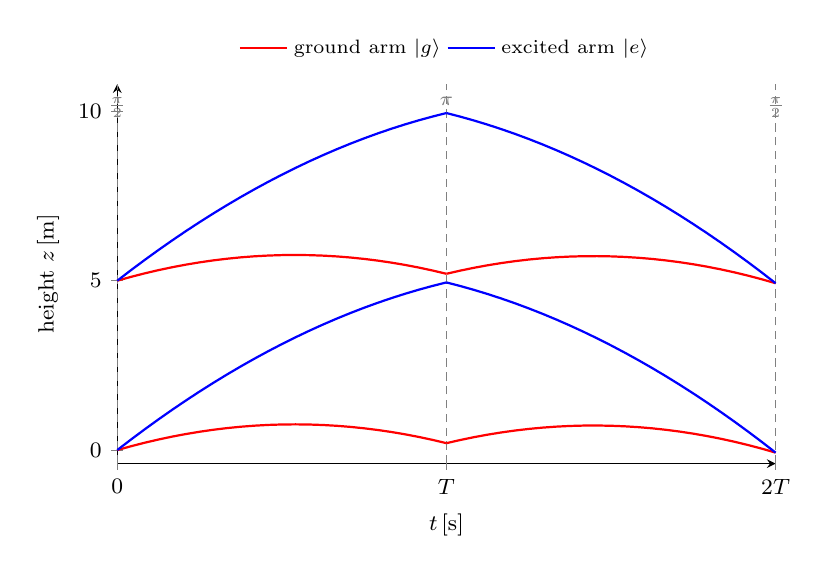
\begin{tikzpicture}
\begin{axis}[
  width=0.82\textwidth, height=6.4cm,
  xlabel={$t$\,[s]}, ylabel={height $z$\,[m]},
  xmin=0, xmax=1.46, ymin=-0.4, ymax=10.8,
  xtick={0,0.73,1.46}, xticklabels={$0$,$T$,$2T$}, ytick={0,5,10},
  axis lines=left, font=\footnotesize,
  legend style={at={(0.5,1.04)},anchor=south,legend columns=2,draw=none,font=\scriptsize},
  clip=false
]
\addplot[densely dashed,gray,forget plot] coordinates {(0,-0.4)(0,10.8)};
\addplot[densely dashed,gray,forget plot] coordinates {(0.73,-0.4)(0.73,10.8)};
\addplot[densely dashed,gray,forget plot] coordinates {(1.46,-0.4)(1.46,10.8)};
\addplot[red,thick,domain=0:0.73,samples=25] {3.86*x - 4.905*x^2};
\addplot[red,thick,domain=0.73:1.46,samples=25,forget plot] {0.2039 + 3.1987*(x-0.73) - 4.905*(x-0.73)^2};
\addplot[blue,thick,domain=0:0.73,samples=25] {10.36*x - 4.905*x^2};
\addplot[blue,thick,domain=0.73:1.46,samples=25,forget plot] {4.9489 - 3.3013*(x-0.73) - 4.905*(x-0.73)^2};
\addplot[red,thick,domain=0:0.73,samples=25,forget plot] {5 + 3.86*x - 4.905*x^2};
\addplot[red,thick,domain=0.73:1.46,samples=25,forget plot] {5 + 0.2039 + 3.1987*(x-0.73) - 4.905*(x-0.73)^2};
\addplot[blue,thick,domain=0:0.73,samples=25,forget plot] {5 + 10.36*x - 4.905*x^2};
\addplot[blue,thick,domain=0.73:1.46,samples=25,forget plot] {5 + 4.9489 - 3.3013*(x-0.73) - 4.905*(x-0.73)^2};
\legend{ground arm $|g\rangle$, excited arm $|e\rangle$}
\node[font=\scriptsize,gray,anchor=north] at (axis cs:0,10.7) {$\tfrac{\pi}{2}$};
\node[font=\scriptsize,gray,anchor=north] at (axis cs:0.73,10.7) {$\pi$};
\node[font=\scriptsize,gray,anchor=north] at (axis cs:1.46,10.7) {$\tfrac{\pi}{2}$};
\end{axis}
\end{tikzpicture}
\caption{Atom trajectories in the gradiometer, computed from the forward model with the
AION-10 parameters (\Cref{tab:params}). Within each interferometer the ground ($|g\rangle$)
and excited ($|e\rangle$) arms separate at the first $\tfrac{\pi}{2}$ pulse, swap momentum at
the $\pi$ pulse and recombine at $2T$; the two interferometers are offset by
$\Delta r=\SI{5}{\metre}$. The propagation phase is the source potential integrated along
these paths.}
\label{fig:trajectories}
\end{figure}

\subsection{The mass model}
\subsubsection{Discretisation elements}
A voxel is the elemental mass unit summed to obtain a body's field; the element is a
strategy behind \texttt{GravitySource}, orthogonal to dynamics and to the far-field path.
\begin{itemize}[leftmargin=*,nosep]
\item \textbf{Point} (v1 default): $V = -Gm/\lVert\rv-\rv_0\rVert$ --- cheapest,
far-field-justified, singular at the element.
\item \textbf{Softened sphere:} $V = -Gm/\sqrt{\lVert\rv-\rv_0\rVert^2 + \varepsilon^2}$ ---
externally near-identical to a point, regularised close in.
\item \textbf{Uniform cube} (Nagy prism~\cite{nagy2000}): the exact closed-form potential of
a homogeneous rectangular prism --- the physically exact voxel, best near the body, costlier
per element.
\end{itemize}

\subsubsection{Field and gradient tensor}
The acceleration and gravity-gradient tensor are
\begin{equation}
\mathbf g = -\grad\Phi,
\qquad
\Gamma_{ij} = \frac{\partial g_i}{\partial x_j} = -\frac{\partial^2\Phi}{\partial x_i\,\partial x_j},
\end{equation}
with $\Phi \equiv V$ the potential per unit mass. By Poisson's equation
$\grad^2\Phi = 4\pi G\rho$, so $\Gamma$ is symmetric and, in vacuum, trace-free
($\tr\Gamma = -4\pi G\rho = 0$) --- a free correctness invariant (\Cref{sec:tests}).

\subsubsection{Multipole expansion (far field)}
Beyond a cutoff distance a rigid body's field is evaluated from its multipole moments,
computed once per body and re-expressed from the pose each tick:
\begin{equation}
\Phi(\rv) = -G\!\left[\frac{M}{r}
+ \frac{\mathbf p\cdot\rhat}{r^2}
+ \frac{1}{2}\frac{\rhat^{\!\top} \mathsf{Q}\,\rhat}{r^3}
+ \cdots\right],
\end{equation}
with monopole $M=\sum_i m_i$, dipole $\mathbf p = \sum_i m_i(\rv_i-\rv_{\mathrm{com}})$
(vanishing about the centre of mass), and quadrupole moment $\mathsf{Q}$. The quadrupole and the
body's \emph{inertia} tensor are linear maps of the same second moment
$\mathsf{C}=\sum_i m_i(\rv_i-\rv_{\mathrm{com}})(\rv_i-\rv_{\mathrm{com}})^{\!\top}$ ---
$\mathsf{Q}=3\mathsf{C}-(\tr\mathsf{C})\mathbb 1$ and $\mathsf{I}=(\tr\mathsf{C})\mathbb 1-\mathsf{C}$
--- so they share principal axes, and the same load-time reduction that yields $\mathsf{Q}$ also
yields the moments that drive free rotation (\Cref{sec:motion}). Near the body the
field reverts to the direct element sum of~\Cref{eq:cloudpot}; the element type matters only
there. The report confirms empirically that sources beyond a few metres are well
approximated as point masses, validating this cutoff.

\begin{figure}[h]
\centering
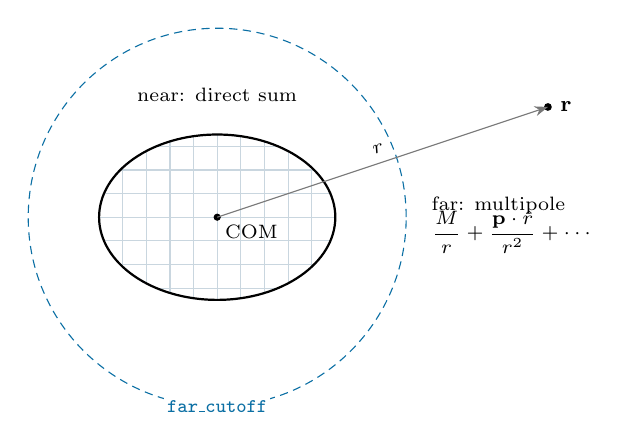
\begin{tikzpicture}[font=\footnotesize]
\coordinate (com) at (0,0);
\begin{scope}
  \clip (com) ellipse (1.5 and 1.05);
  \draw[step=0.3,draw=rule] (-1.8,-1.2) grid (1.8,1.2);
\end{scope}
\draw[thick] (com) ellipse (1.5 and 1.05);
\fill (com) circle (1.3pt); \node[below right=-1pt of com]{\scriptsize COM};
\draw[densely dashed,draw=seam] (com) circle (2.4);
\node[seam,font=\scriptsize,fill=white,inner sep=1pt] at (0,-2.4){\texttt{far\_cutoff}};
\coordinate (P) at (4.2,1.4);
\fill (P) circle (1.4pt); \node[right=1pt of P]{$\rv$};
\draw[->,>=Stealth,draw=cmt] (com) -- node[sloped,above,font=\scriptsize]{$r$} (P);
\node[align=center,font=\scriptsize] at (0,1.55) {near: direct sum};
\node[align=left,font=\scriptsize,anchor=west] at (2.6,-0.1)
  {far: multipole\\[-2pt]$\dfrac{M}{r}+\dfrac{\mathbf p\cdot\hat r}{r^2}+\cdots$};
\end{tikzpicture}
\caption{Voxelisation and the near/far split. A body is filled with mass elements (the voxel
cloud). At a field point $\rv$ within \texttt{far\_cutoff} the potential is the direct element
sum (\Cref{eq:cloudpot}); beyond it, the body's multipole moments suffice. The discretisation
element matters only in the near region.}
\label{fig:voxel}
\end{figure}

\subsection{Analytic primitives (the oracle)}
\label{sec:oracle}
Closed-form / quadrature potentials of homogeneous primitives are the reference the voxel
cloud is validated against; they are \emph{not} used in generation. For a cylinder of mass
$m$, radius $R$, height $H$~(122),
\begin{equation}
V(\rv) = -\frac{G m}{\pi R^2 H}
\int_{-H/2}^{H/2}\!\!\int_{0}^{R}\!\!\int_{0}^{2\pi}
\frac{r'\dd\theta\dd r'\dd h'}
{\sqrt{(D-D_0-r'\cos\theta)^2 + (w-w_0-r'\sin\theta)^2 + (h-h_0-h')^2}},
\end{equation}
and for a cuboid of side lengths $a,b,c$~(121),
\begin{equation}
V(\rv) = -\frac{G m}{abc}
\int\!\!\int\!\!\int_{\text{box}}
\frac{\dd w'\dd h'\dd D'}{\sqrt{(D-D')^2 + w'^2 + (h-h')^2}} ,
\end{equation}
with the planar sheet~(118/119) the $c\to 0$ surface analogue. A voxelised primitive must
converge to these as $\texttt{voxel\_size}\to 0$ --- the proof that the voxel approach is
correct.

\subsection{Quasi-static limit (sanity check only)}
For a uniform field the single-interferometer response reduces to the closed form~(51)
\begin{equation}
\Delta\phi \approx k_{\mathrm{eff}}\, a\, T^2 ,
\end{equation}
retained only as a uniform-field cross-check. GGN sources are non-uniform, so
\Cref{eq:singlephi} is the model.

\subsection{The ULDM signal (common-mode channel)}
\label{sec:uldm}
The scientific target is a coherent, closed-form phase --- not a gravitational source at all,
but an oscillation of the atomic transition frequency driven by a scalar dark-matter field.
It is additive to the GGN signal and identical across the array (\Cref{sec:array}). For a
gradiometer of baseline $L$ and separation $\Delta r$ with $n$ LMT kicks~\cite{arvanitaki2015},
\begin{equation}
\Delta\Phi_\phi(t) = 8\,\frac{\delta\omega_A}{\omega_\phi}\,\frac{\Delta r}{L}\,
\sin\!\frac{\omega_\phi n L}{2c}\;
\sin\!\frac{\omega_\phi\big(T-(n{-}1)L/c\big)}{2}\;
\sin\!\frac{\omega_\phi T}{2}\;
\cos\!\Big(\omega_\phi\big(\tfrac{2T+L/c}{2}+t\big)+\theta\Big),
\label{eq:uldm}
\end{equation}
with $\omega_\phi = 2\pi f_\phi$ and the transition-frequency modulation amplitude
\begin{equation}
\delta\omega_A = \omega_A\,\sqrt{4\pi G_{\mathrm N}}\,
\big(d_{m_e} + (2+\xi)\,d_e\big)\,\frac{\sqrt{2\rho_\phi}}{m_\phi}\,\kappa,
\end{equation}
where $\omega_A$ is the atomic transition frequency, $d_e, d_{m_e}$ the dilatonic couplings,
$\xi$ the clock-transition coefficient, $\rho_\phi$ the local dark-matter density, $m_\phi$ the
scalar mass, $G_{\mathrm N}$ Newton's constant in natural units, and $\kappa$ a unit
conversion (\Cref{tab:uldm}). The oscillation frequency is set by the particle mass:
$f_\phi = m_\phi c^2/h$ (and $\SI{4e-16}{\electronvolt}\to\SI{0.097}{\hertz}$), so
\emph{recovering the line is measuring the dark-matter mass}. Because \Cref{eq:uldm} is cheap
and deterministic, it is evaluated directly rather than through the gravity kernel; in a
scenario it is the common-mode channel the Gradar tracker (\Cref{sec:radar}) learns to reject
and the line the analysis pipeline (\Cref{sec:freq}) recovers.

\subsection{Frequency domain}
\label{sec:freq}
The signal is naturally analysed as a periodogram. On a \emph{uniform} grid this is the
discrete spectrum~(66),
\begin{equation}
S_k = \frac{\Delta t}{N}\left|\sum_{\ell=0}^{N-1}\Delta\Phi_\ell\,
e^{-2\pi i \ell k / N}\right|^2,
\qquad f_k = \frac{k}{N\Delta t},
\end{equation}
with Nyquist frequency $f_{\mathrm N} = 1/(2\Delta t)$ and resolution $\Delta f =
1/(N\Delta t)$. Oscillating sources produce peaks at integer multiples $n f_0$ (from the
nonlinearity of $V$), with mass-independent peak-height ratios; harmonics above $f_{\mathrm N}$
mirror back.

\textbf{The realistic schedule is non-uniform, so the FFT does not apply.} Cycle jitter,
shot failures and scheduled gaps (\Cref{sec:schedule}) leave the measurement times
$\{t_\ell\}$ irregular, on which the FFT --- which assumes even spacing --- produces spurious
structure. The correct estimator is the \textbf{Lomb--Scargle periodogram}, which fits
sinusoids by least squares at each trial frequency and handles arbitrary sampling:
\begin{equation}
S(f) = \frac{1}{2}\!\left[
\frac{\big(\sum_\ell y_\ell\cos\omega(t_\ell-\tau)\big)^2}{\sum_\ell\cos^2\omega(t_\ell-\tau)}
+\frac{\big(\sum_\ell y_\ell\sin\omega(t_\ell-\tau)\big)^2}{\sum_\ell\sin^2\omega(t_\ell-\tau)}
\right],
\end{equation}
$\omega = 2\pi f$, with the offset $\tau$ fixing time-shift invariance~\cite{scargle1982}. The
Lomb--Scargle transform is the first-class spectral output; the uniform FFT is retained as the
fast path for the degenerate evenly-sampled case. GGN removal before reading the ULDM line is a
\emph{least-squares notch} at each oscillator frequency \emph{and its second harmonic} (the
harmonic because a large-amplitude oscillation is anharmonic, \Cref{sec:freq} and the pendulum
of \Cref{sec:motion}); a robust detection floor is the median of $\sqrt{S}$ off the peak.

\subsection{The two time scales}
The within-flight integration step $\texttt{fine\_dt}\approx\SI{0.01}{\second}$ evaluates
each $\delta\phi$ over the flight $2T = \SI{1.46}{\second}$; the measurement cadence
$\Delta t = \SI{2}{\second}$ is the spacing at which $\Delta\Phi_\ell$ is sampled (it sets
$f_{\mathrm N}$ and the spectral mirroring). These are distinct axes and must not be
conflated.

\begin{figure}[h]
\centering
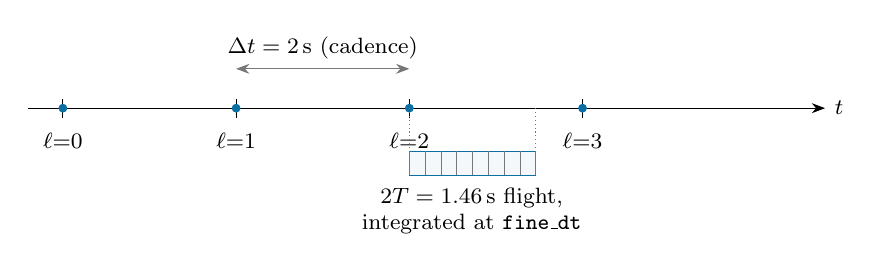
\begin{tikzpicture}[font=\footnotesize,x=2.2cm]
\draw[->,>=Stealth] (-0.2,0) -- (4.4,0) node[right]{$t$};
\foreach \l in {0,1,2,3}{
  \draw (\l,0.12) -- (\l,-0.12);
  \node[below=2pt] at (\l,-0.12){$\ell{=}\l$};
  \fill[seam] (\l,0) circle (1.6pt);
}
\draw[<->,>=Stealth,draw=cmt] (1,0.5) -- (2,0.5) node[midway,above]{$\Delta t=\SI{2}{\second}$ (cadence)};
\draw[fill=boxbg,draw=seam] (2,-0.55) rectangle (2.73,-0.85);
\foreach \i in {0,1,...,8}{\draw[draw=cmt,line width=0.3pt] ({2+\i*0.0913},-0.55) -- ({2+\i*0.0913},-0.85);}
\node[below=1pt,align=center] at (2.36,-0.85){$2T=\SI{1.46}{\second}$ flight,\\ integrated at \texttt{fine\_dt}};
\draw[draw=cmt,densely dotted] (2,0)--(2,-0.55);
\draw[draw=cmt,densely dotted] (2.73,0)--(2.73,-0.55);
\end{tikzpicture}
\caption{The two time scales. Measurements are spaced by the cadence
$\Delta t=\SI{2}{\second}$ (which sets $f_{\mathrm N}=1/2\Delta t$); each $\Delta\Phi_\ell$ is
itself a phase integrated over a $2T=\SI{1.46}{\second}$ atom flight at the fine step
\texttt{fine\_dt}. The flight is shorter than the cadence --- the remainder is dead time.}
\label{fig:timescales}
\end{figure}

\subsection{Measurement schedule and contamination}
\label{sec:schedule}
A real run is not an unbroken uniform series; the measurement times carry structure that the
analysis (\Cref{sec:freq}) and the Gradar front-end (\Cref{sec:radar}) must contend with, so
the schedule is modelled explicitly and the bundle carries the actual $\{t_\ell\}$ rather than
assuming a uniform $\Delta t$. Four effects, each seedable, compose:
\begin{itemize}[leftmargin=*,nosep]
\item \textbf{Cycle jitter} --- the cycle duration varies (e.g.\ $T_c\sim\mathcal U(1.9,3.0)$\,s,
or a per-shot $\pm$ offset), so $\{t_\ell\}$ is non-uniform.
\item \textbf{Shot failures} --- each measurement is dropped independently with probability
$p_{\text{fail}}$ (MOT/preparation failure).
\item \textbf{Scheduled gaps} --- the device runs only on a duty schedule (e.g.\ nighttime),
with jitter on the switch times, leaving daily gaps over multi-day runs.
\item \textbf{Transient events} --- large near-field disturbances (a lift: a heavy mass on a
clipped vertical pass) arrive as a Poisson process and contaminate the cycles they overlap;
these are \emph{tagged} so they can be excised (with padding) or handed to the model as a
contamination mask.
\end{itemize}
The uniform, gap-free, failure-free series is the degenerate default. The lift is just a
\texttt{Lift} motion (\Cref{sec:motion}) flagged as a transient; excision is a mask over the
cadence axis, not a physics change.

\subsection{Noise model}
The clean signal is corrupted by an ordered, seedable stack:
\begin{equation}
\sigma_\phi \approx \frac{1}{C\sqrt{N_{\text{atoms}}}}\quad(\text{atom shot noise}),
\end{equation}
with $C$ the fringe contrast, plus a vibration residual with a gradiometer common-mode
rejection ratio. Noise is additive realism layered after the forward model is validated.

\subsection{Atmospheric gravity-gradient noise}
\label{sec:atmo}
Beyond discrete moving masses, the dominant low-frequency GGN in a vertical interferometer is
\emph{distributed and stochastic}: fluctuations in the density of the air above the instrument
perturb the local potential. Carlton \emph{et al.}~\cite{carlton2025} give the first
characterisation for vertical AIs, in exactly Cavendish's \SIrange{0.01}{1}{\hertz} band --- the
ULDM line at \SI{0.1}{\hertz} sits inside it. The key structural point: it enters through the
\emph{same} potential integral as a rigid body (\Cref{sec:forward,fig:voxel}); only the source
is a realised random density field $\delta\rho$ rather than a voxel cloud. So atmospheric GGN
is ``a source whose mass distribution is a stochastic field,'' and the existing gravity kernel
and forward model evaluate it unchanged --- it is the principal growth target for the otherwise
placeholder noise stack.

Two channels, each mapping a fluctuation to a density perturbation $\delta\rho/\rho_0$ and
thence to a vertical acceleration on the arms:
\begin{itemize}[leftmargin=*,nosep]
\item \textbf{Infrasound (pressure).} Adiabatic, $\delta\rho/\rho_0 = \delta p/(\gamma p_0)$,
modelled as plane waves reflecting off the half-space surface at incidence $\theta$; this gives
a \emph{closed-form} vertical acceleration and per-shot phase (cheap, like the ULDM signal).
Amplitudes come from the global high/low ambient-infrasound models (Bowman; Kristoffersen),
with a typical $\delta p\sim\SI{e-3}{}$~mbar and strong (up to two-decade) seasonal variation.
\item \textbf{Temperature (turbulence).} $\delta\rho/\rho_0 = \delta T/T_0$, from thermal eddies
in the surface boundary layer advected past the tower at wind speed $U$ (Taylor's
frozen-turbulence hypothesis, $k_x = \omega/U$). The eddy wavenumber spectrum takes the
Greenwood--Tarazano form $\Phi(k)\propto (k^2 + k/\Lambda)^{-11/6}$ (Kolmogorov $k^{-11/3}$ in
the inertial subrange, corrected at low frequency), outer scale $\Lambda$ at the Obukhov length;
the resulting PSD is numerical, with no closed form.
\end{itemize}

\textbf{Gradiometer and array structure.} Unlike a horizontal LIGO-like pair, the two clouds of
a \emph{vertical} gradiometer feel \emph{correlated} atmospheric noise along the baseline, so the
double-difference partially rejects it --- the noise is the subtracted spectrum
$S_g(f,z_0)-S_g(f,z_0+\Delta z)$, and the cloud nearest the surface dominates. Crucially for the
array (\Cref{sec:array}), atmospheric GGN has a finite \emph{spatial correlation length} --- the
infrasound wavelength ($\approx\SI{343}{\metre}$ at \SI{1}{\hertz}) and the eddy/outer scale
($\sim\SI{170}{\metre}$) --- so across horizontally separated detectors it is only
\emph{partially} correlated. This places it between the two limits the array already exploits:
fully common-mode (ULDM, coherent over astronomical scales) and fully local (a nearby mass). The
array's spatial sampling is therefore what separates all three regimes, and this distributed
background is the realistic floor the Gradar front-end (\Cref{sec:radar}) must detect through.
\textbf{Depth} is the passive mitigation: temperature noise falls off sharply with $z_0$, while
vertically incident infrasound penetrates furthest.

The transfer from acceleration to gradiometer phase is the sequence's own response
$T_\phi = 2 n \kappa L \cos(\omega T)\sin^2(\omega T/2)$ (LMT order $n$, laser wavevector
$\kappa=\omega_a/c$), which Cavendish's forward model already embodies; its zeros notch the noise
at interrogation-time--dependent frequencies. \Cref{tab:atmo} lists the parameters.

\begin{table}[h]
\centering
\caption{Atmospheric GGN parameters~\cite{carlton2025}.}
\label{tab:atmo}
\small
\begin{tabular}{@{}lll@{}}
\toprule
Symbol & Quantity & Value \\
\midrule
$\rho_0$  & mean air density                 & \SI{1.3}{\kilogram\per\cubic\metre}\\
$p_0$     & mean pressure                    & $\num{1013}$~mbar\\
$\gamma$  & adiabatic index (air)            & \num{1.4}\\
$T_0$     & mean air temperature             & \SI{300}{\kelvin}\\
$c_T$     & temperature structure constant   & $\num{0.2}\ \mathrm{K^2\,m^{-2/3}}$\\
$\Lambda$ & turbulence outer scale (Obukhov) & $\sim\SI{170}{\metre}$\\
$U$       & mean wind speed                  & $\sim\SI{20}{\metre\per\second}$\\
$\delta p$& typical infrasound amplitude     & $\sim\num{e-3}$~mbar\\
band      & relevant frequencies             & \SIrange{0.01}{1}{\hertz}\\
\bottomrule
\end{tabular}
\end{table}

\subsection{Reference parameters}
\Cref{tab:params} lists the AION-10 defaults; \Cref{tab:anchors} the published
regression targets; \Cref{tab:uldm} the dark-matter signal parameters. The clock isotope is
$^{87}$Sr (the \SI{698}{\nano\metre} clock transition fixes this). The mass
$m_A=\num{1.46e-25}$ is a fixed calibration constant supplied by collaborators --- the
natural-abundance (isotopic-mixture) value, $\approx 87.6\,\mathrm{u}$, not
$^{87}$Sr's single-isotope \num{1.443e-25}. Cavendish keeps this value to reproduce the
oracle; the forward model is linear in $m_A$, so the ${\sim}1\%$ difference is immaterial.

\begin{table}[h]
\centering
\caption{AION-10 instrument defaults (from~\cite{parish2026} and reference code).}
\label{tab:params}
\small
\begin{tabular}{@{}llll@{}}
\toprule
Symbol & Quantity & Value & \\
\midrule
$G$               & gravitational constant   & \num{6.67430e-11} & \unit{\cubic\metre\per\kilogram\per\second\squared}\\
$m_A$             & atomic mass ($^{87}$Sr)  & \num{1.46e-25}    & \unit{\kilogram}\\
$\hbar$           & reduced Planck constant  & \num{1.055e-34}   & \unit{\joule\second}\\
$\lambda$         & clock wavelength         & \num{698e-9}      & \unit{\metre}\\
$k$               & wavenumber $2\pi/\lambda$& $\approx\num{9.0e6}$ & \unit{\per\metre}\\
$T$               & pulse separation         & \num{0.73}        & \unit{\second}\\
$2T$              & flight time              & \num{1.46}        & \unit{\second}\\
$n_{\mathrm{kick}}$ & photon kicks (LMT)     & \num{1000}        & ---\\
$v_{\mathrm{rec}}$  & recoil/arm velocity    & $\approx\num{6.5}$ & \unit{\metre\per\second}\\
$g$               & local gravity            & \num{9.81}        & \unit{\metre\per\second\squared}\\
$\Delta r$        & baseline (IFO separation)& \num{5}           & \unit{\metre}\\
                  & tower height             & \num{10}          & \unit{\metre}\\
$u_0$             & launch velocity          & \num{3.86}        & \unit{\metre\per\second}\\
$\Delta t$        & measurement cadence      & \num{2}           & \unit{\second}\\
$\texttt{fine\_dt}$ & integration step       & \num{0.01}        & \unit{\second}\\
\bottomrule
\end{tabular}
\end{table}

\begin{table}[h]
\centering
\caption{Published GGN regression targets (numerical oracle).}
\label{tab:anchors}
\small
\begin{tabular}{@{}lll@{}}
\toprule
Source & Scenario & Peak $|\Delta\Phi|$ \\
\midrule
Point mass        & \SI{10}{\kilogram}, $D=\SI{10}{\metre}$, vertical pass \SI{2.5}{\metre\per\second} & $\approx \SI{7}{\milli\radian}$ \\
Point oscillator  & \SI{1}{\kilogram}, $D_0=\SI{5}{\metre}$, $h=1+\cos(2\pi\cdot 0.1\,t)$           & $\approx \SI{2}{\milli\radian}$ \\
Concrete wall (cuboid) & $0.225\times 6.1\times \SI{12.2}{\metre}$, \SI{0.1}{\hertz}, \SI{1}{\micro\metre} & $\approx \SI{50}{\micro\radian}$ \\
AION scaffold (cylinders) & multiple members, \SI{0.2}{\hertz}, \SI{1}{\micro\metre}                 & $\approx \SI{10}{\micro\radian}$ \\
\bottomrule
\end{tabular}
\end{table}

\begin{table}[h]
\centering
\caption{Dark-matter (ULDM) signal parameters for \Cref{eq:uldm} (from the reference code).}
\label{tab:uldm}
\small
\begin{tabular}{@{}llll@{}}
\toprule
Symbol & Quantity & Value & \\
\midrule
$m_\phi$        & scalar (ULDM) mass            & \num{4e-16}    & \unit{\electronvolt}\\
$f_\phi$        & oscillation freq.\ $m_\phi c^2/h$ & $\approx\num{0.1}$ & \unit{\hertz}\\
$\rho_\phi$     & local dark-matter density     & \num{0.3}      & \unit{\giga\electronvolt\per\cubic\centi\metre}\\
$\omega_A$      & atomic transition frequency   & \num{2.67e15}  & \unit{\radian\per\second}\\
$d_e,\ d_{m_e}$ & dilatonic couplings           & \num{1}        & ---\\
$\xi$           & clock-transition coefficient  & \num{0.06}     & ---\\
$\theta$        & initial phase                 & $\pi/2$        & \unit{\radian}\\
$G_{\mathrm N}$ & Newton constant (natural units) & \num{6.708e-39} & \unit{\per\giga\electronvolt\squared}\\
$\kappa$        & unit conversion (nat.\ $\to$ SI) & \num{2.77e-12} & ---\\
\bottomrule
\end{tabular}
\end{table}

\section{Gradar: the Inference Target}
\label{sec:radar}

Cavendish is the data engine for \emph{Gradar}: a learned tracker that recovers
the time-resolved tracks of moving masses from the array signal. The tracker itself is
downstream (deferred), but its target is what fixes the label, the prior and the analysis
outputs, so it is specified here.

\subsection{Tracking, not static localisation}
The task is tracking, not a single fix: a mass moves through the array's field of view and its
track --- position over time, hence velocity and trajectory --- is reconstructed from how the
gradient signature sweeps across the detectors. \textbf{The motion is the information}: a
stationary mass gives one geometry, a moving one sweeps through many, and that temporal
diversity is what makes the inverse well-posed (the same reason a single-axis gradiometer can
recover a trajectory at all). It is \emph{passive} --- nothing is emitted; the masses' own
static fields are read as they move, so there is no time-of-flight ranging, and range comes
from amplitude and the cross-detector triangulation of \Cref{sec:array}. The array is a phased
gravimetric aperture; the tracker is the inference over it.

\subsection{Why a JEPA}
The target maps onto a temporal joint-embedding predictive architecture: past
gradient-signature windows predict the latent of future windows, so the latent must encode the
sources' kinematic state because that state generates the next window. A world-model latent is
literally ``predict where it will be'' --- tracking. The ladder is supervised single-target
tracker $\to$ temporal JEPA (masked-future prediction, a probe reading off the track) $\to$
world-model tracker (online). The multi-detector signal is the natural multi-channel input,
and the cross-channel structure --- common-mode for ULDM, differential for GGN, ratios and
timings for position --- is exactly what the representation should capture.

\subsection{Where the difficulty (and the experiment) lives}
\begin{itemize}[leftmargin=*,nosep]
\item \textbf{Multi-target data association.} Several masses superpose \emph{linearly} in the
field --- trivial to simulate (add the clouds) --- but their tracks must be disentangled from
the summed signal. Linearity helps the forward model and nothing in the inverse; the unmixing
is the hard part, the classical radar-tracker (Kalman/JPDA) problem where a learned tracker can
win.
\item \textbf{Degeneracy broken by motion.} A heavy/slow/far mass and a light/fast/near one can
\emph{momentarily} alias, but their tracks diverge, so tracking over time resolves what a
snapshot cannot. The dedicated confusion-pair prior (\Cref{sec:components}) --- instantaneously
degenerate pairs --- is the clean test of whether the world-model actually uses time.
\item \textbf{Detection before tracking.} Whether a target is present at all, under the GGN and
the schedule gaps, makes the measurement schedule (\Cref{sec:schedule}) the Gradar front-end
rather than an afterthought.
\end{itemize}

\subsection{What the signal recovers: the identifiability ladder}
\label{sec:identif}
The exterior field is a multipole series, and recoverability falls off with moment order, so
the expansion already in the model (\Cref{fig:voxel}) \emph{is} the identifiability ladder:
``what can be recovered'' is answered moment by moment, not all at once.

\textbf{Trajectory and total mass (monopole).} The centre-of-mass motion lives entirely in the
monopole --- the strongest, slowest-falling term --- so position over time, hence velocity, is
the robust content; total mass is the monopole strength, recoverable but mass--distance
degenerate for a single device and disambiguated by the array (\Cref{sec:array}).

\textbf{Shape, and exactly how hard (quadrupole).} The dipole vanishes about the centre of
mass, so shape onsets at the quadrupole, and the quadrupole/monopole signal ratio scales as
$(a/r)^2$ in source size $a$ and distance $r$ --- invariant whether $V$, $\mathbf g$ or
$\Gamma$ is measured, since the extra $1/r$ powers cancel in the ratio. That single number is
the entire shape-SNR budget: order-unity for the scaffold (members and distances both
metre-scale), negligible for a distant lift. The T2.4 departure-from-monopole sweep
(\Cref{tab:tests}) is the forward map of this budget.

\textbf{Interior density is unrecoverable in principle.} The exterior inverse problem is
non-unique: a uniform shell is identical to a point mass, and interior mass can be
redistributed across an equivalence class without changing any external moment. Free-form
(voxel) density reconstruction is therefore \emph{impossible}, not merely ill-conditioned ---
no SNR or baseline recovers what the field does not carry.

\textbf{Shape as model selection.} Restricting to a shape family is the regulariser that makes
the inverse well-posed: it selects one representative of the equivalence class. The target is
thus \emph{model selection} over a dictionary (sphere, cylinder, cuboid, sheet) with pose and
scale, not field inversion --- finite-dimensional, well-posed, and asking only for the low
moments that are recoverable at all. The dictionary is the engine's own parameterised body
library, so the inference target and the generative prior are the same object, and the shape
label is a library entry plus parameters rather than a new representation; for the JEPA this is
a shape-class posterior with continuous moment regression.

\textbf{The moments close the geometry.} The shape prior does more than classify. For a uniform
cylinder the quadrupole fixes only the elongation combination $\mathsf{Q}_{zz}\propto H^2-3R^2$;
adding the class and a uniform-density assumption closes the system --- the monopole gives
$M=\rho\pi R^2 H$ and the quadrupole gives $H^2-3R^2$, two equations for $(R,H)$. The aspect
ratio $H=\sqrt3\,R$ gives $\mathsf{Q}_{zz}=0$, a cylinder indistinguishable from a sphere at
quadrupole order --- a genuine blind spot. A single vertical gradiometer reads one projection of
$\Gamma$, hence of $\mathsf{Q}$, giving elongation magnitude only; the array samples
$\mathsf{Q}$ from several bearings, reconstructing the full tensor whose eigenvectors are the
principal axes --- so orientation becomes observable, ``it is elongated'' sharpening to ``it is
a cylinder pointing that way.'' None of this repeals $(a/r)^2$.

\textbf{Rotation isolates the quadrupole.} A source rotating about a fixed centre of mass
(\Cref{sec:motion}) holds the monopole fixed and the dipole zero, so its time-varying signal is
\emph{purely} quadrupole-and-higher --- the exact complement of monopole-dominated translation,
and the cleanest available probe of this rung. A freely tumbling asymmetric body goes further:
since its inertia and quadrupole tensors share principal axes, the flip dynamics and the static
shape signature are two views of one tensor, and the body over-constrains its own geometry.

\textbf{Velocity} is the derivative of the recovered track, so its limits are temporal: the
within-flight smear (each $\Delta\Phi_\ell$ is a \SI{1.46}{\second} integral, so motion
\emph{during} a flight blurs) and the \SI{2}{\second} cadence --- ample for \SI{0.1}{\hertz}
GGN, a wall for anything fast.

\begin{table}[h]
\centering
\caption{The recoverability ladder: what the signal carries, by multipole order.}
\label{tab:identifiability}
\small
\begin{tabular}{@{}p{0.30\textwidth}p{0.27\textwidth}p{0.35\textwidth}@{}}
\toprule
Content & Source & Status \\
\midrule
Position over time, velocity & monopole (CoM motion) & robust, array-aided \\
Total mass & monopole strength & recoverable; mass--distance degenerate, broken by the array \\
Elongation magnitude & quadrupole, one projection & marginal --- the $(a/r)^2$ budget \\
Orientation, shape moments & full $\mathsf{Q}$ tensor & array only; still $(a/r)^2$-limited \\
Geometry $(R,H)$, known class & monopole $+$ quadrupole $+\ \rho$ & closes \emph{given} the shape prior \\
Interior density $\rho(\xv)$ & --- & impossible in principle \\
\bottomrule
\end{tabular}
\end{table}

\subsection{Two channels, one array; and the identifiability floor}
Gradar and ULDM detection are not competing framings but the differential and
common-mode halves of the same multi-channel problem (\Cref{sec:array}): the tracker works the
differential structure and rejects the common-mode ULDM; the dark-matter search works the
common mode and rejects the differential GGN. The rigorous ceiling on both is the
Fisher-information / Cram\'er--Rao bound, computed from the differentiable forward model
(\Cref{nfr:diff}): the track (position and velocity) covariance given the array geometry and
SNR; the quadrupole detectability that sets whether shape is accessible at all (the $(a/r)^2$
budget of \Cref{sec:identif}) and the model-selection power between shape classes; and a
multi-target resolvability measure. A tracker is then judged against this floor, and array
placement is optimised against it.

\section{Requirements}
\label{sec:req}

\subsection{Functional requirements}

\begin{freq}[Mesh import and voxelisation]
The system shall construct source mass clouds from analytic primitives (sphere, shell, cuboid,
cylinder, and unions thereof, each with closed-form moments as a validation oracle) and from
imported triangle meshes (explicit scale; no unit guessing) discretised at a configurable
resolution \texttt{voxel\_size}, with a configurable element kind (point, softened sphere, cube).
Every produced cloud shall have exact total mass (renormalised), its centre of mass at the
body-frame origin (zero dipole), and a deterministic element order. Open or non-manifold meshes
shall be classified robustly (generalised winding numbers) with a diagnostic, failing loudly when
the interior is ambiguous.
\end{freq}

\begin{freq}[Gravity evaluation]
The system shall evaluate the gravitational potential $V$, acceleration $\mathbf g$ and
gradient tensor $\Gamma$ at arbitrary world points for single elements, for a voxel cloud,
and for analytic primitives, routing near-field points to a direct element sum and
far-field points to a multipole expansion.
\end{freq}

\begin{freq}[Analytic oracle primitives]
The system shall provide homogeneous sphere, cuboid, cylinder and sheet primitives with
closed-form or quadrature potentials, for validating the voxel cloud (\Cref{sec:tests}).
These shall not be used in signal generation.
\end{freq}

\begin{freq}[Rigid source dynamics]
The system shall represent a rigid body as a body-frame cloud plus a continuous pose
trajectory $\texttt{pose\_at}(t)$, built from a path, a timing law, an orientation law and a
rigid placement (\Cref{sec:motion}), with named motions covering at minimum static, linear
pass, oscillation, circular, lift, pendulum, and rotation (spin, rocking, and the free-rotation
Euler top), composable by superposition and by time-sequencing.
\end{freq}

\begin{freq}[Composite and multi-target sources]
The system shall represent a scene as a superposition of independent sources, summing their
clouds (gravity is linear). This shall support the multi-cylinder scaffold case and
\emph{multiple simultaneous moving targets}, each with its own trajectory, as the multi-target
Gradar scenario.
\end{freq}

\begin{freq}[Instrument and arm construction]
The system shall model the AION-10 gradiometer and construct the four parabolic arm
trajectories with LMT recoil (\Cref{sec:traj}), caching them as interpolable paths over
$[0,2T]$, with all parameters of \Cref{tab:params} configurable.
\end{freq}

\begin{freq}[Detector array]
The system shall model an array of gradiometers at configurable ground placements
(\Cref{sec:array}), evaluating the forward model independently per detector and emitting one
differential-phase channel per detector, such that $N{=}1$ reproduces a single gradiometer and
the placement geometry is a free parameter (and an analysis knob, \Cref{sec:radar}).
\end{freq}

\begin{freq}[ULDM signal]
The system shall provide the closed-form coherent dark-matter phase (\Cref{eq:uldm}) as an
additive, common-mode signal applied identically across the array, with the parameters of
\Cref{tab:uldm} configurable, and shall be able to enable or disable it per scenario.
\end{freq}

\begin{freq}[Forward model]
The system shall compute the differential phase $\Delta\Phi_\ell$ via the propagation-phase
double-difference integral (\Cref{eq:singlephi,eq:doublediff}), querying the source position
at \texttt{fine\_dt} resolution within each flight. A quasi-static gradient model shall be
available as an alternative for uniform-field cross-checks.
\end{freq}

\begin{freq}[Sampling and Nyquist]
The system shall sample the signal at the measurement cadence \texttt{cycle\_time}, and
expose enough metadata that periodograms and Nyquist mirroring are computed correctly.
\end{freq}

\begin{freq}[Measurement schedule]
The system shall optionally apply a seedable measurement schedule (\Cref{sec:schedule}) ---
cycle jitter, independent shot failures, scheduled (duty-cycle) gaps, and Poisson transient
events --- producing a non-uniform set of measurement times $\{t_\ell\}$ carried explicitly in
the bundle, with transient-contaminated cycles tagged for excision or masking. A uniform,
gap-free schedule shall be the default.
\end{freq}

\begin{freq}[Noise stack]
The system shall apply an ordered, seedable stack of additive noise sources (at minimum
atom shot noise and a vibration residual) to the clean signal, deterministic given the seed.
\end{freq}

\begin{freq}[Atmospheric gravity-gradient noise]
The system shall provide atmospheric GGN (\Cref{sec:atmo}) as a physically-modelled noise
source --- an infrasound (pressure) channel and a temperature (turbulence) channel, each
realised as a stochastic density field through the gravity kernel and differenced across the
baseline --- with the parameters of \Cref{tab:atmo} and the detector depth $z_0$ configurable.
\end{freq}

\begin{freq}[State bundle output]
The system shall emit the full per-measurement state bundle (\Cref{tab:bundle}) with a leading
measurement-cadence time axis, a per-detector signal channel, and the time-resolved source
tracks. The \emph{complete} record is the default; \emph{field selection} (computing a field only
when requested) is a cost/storage optimisation, never a change to what the bundle means or to any
imposed task.
\end{freq}

\begin{freq}[Track ground truth]
The system shall emit, as ground truth, the time-resolved track of every source (position over
time, hence velocity and trajectory) and the target count; for multiple targets this is a set of
tracks. A supervised Gradar tracker (\Cref{sec:radar}) would use these as its target, but the
engine emits them as ground-truth fields and imposes no such role.
\end{freq}

\begin{freq}[Signal decomposition and shape descriptors]
The system shall optionally emit the per-channel ground-truth decomposition of \texttt{signal} ---
the phase from target masses, from atmospheric GGN, from ULDM, and the additive measurement noise,
which sum to \texttt{signal} --- and the per-interferometer phases before the double-difference.
It shall optionally emit the static per-source shape descriptors (mass, inertia tensor, principal
moments and axes, gravitational quadrupole), all derived from \texttt{source\_cloud}. These are
\emph{optional} cost choices, not changes to the bundle's meaning.
\end{freq}

\begin{freq}[Single and streaming evaluation]
The system shall provide \texttt{run} (one explicit scenario, returning one bundle) and
\texttt{stream} (an endless prior-sampled iterable yielding batched bundles).
\end{freq}

\begin{freq}[Derived outputs]
The system shall provide the Lomb--Scargle periodogram (\Cref{sec:freq}) as a first-class
derived field for non-uniformly sampled series, with the uniform FFT as the fast path for
evenly-sampled data.
\end{freq}

\begin{freq}[Identifiability analysis]
The system shall, using the differentiable forward model (\Cref{nfr:diff}), expose the
Fisher-information / Cram\'er--Rao bound on the recoverable source parameters --- the track
(position and velocity) covariance given the array geometry and SNR, the quadrupole
detectability and shape-class model-selection power (\Cref{sec:identif}), and a multi-target
resolvability measure (\Cref{sec:radar}).
\end{freq}

\begin{freq}[Configuration and reproducibility]
The system shall expose a single typed configuration schema to both the SDK (dataclasses)
and CLI (TOML/YAML $+$ flag overrides) with no duplicated parameter list, such that
$(\text{config},\text{seed})$ fully determines a run.
\end{freq}

\begin{freq}[Python SDK]
The system shall provide a Python package (maturin/PyO3 over \texttt{sim-core}) returning
torch-ready tensors, runnable inside \texttt{DataLoader} workers with the GIL released
during compute and prefetch enabled.
\end{freq}

\begin{freq}[Command-line interface]
The system shall provide a console entry point wrapping \texttt{run}/\texttt{stream} for
producing deliberately frozen bundles (shared eval sets, caches).
\end{freq}

\begin{freq}[Viewer]
The system shall provide a native viewer rendering signal and periodogram traces and a 3D
scene (baseline, atom clouds, source body on its trajectory), source-agnostic so that a
model prediction can be overlaid on ground truth.
\end{freq}

\begin{freq}[Optional persistence]
The system shall optionally serialise bundles tensor-natively (e.g.\ safetensors /
WebDataset; Zarr/HDF5 for volumetric fields) for a frozen cache, outside the training loop.
\end{freq}

\subsection{Non-functional requirements}

\begin{nfreq}[Accuracy]
On the point-mass anchors of \Cref{tab:anchors} the system shall reproduce the oracle to
$\geq 99\%$; voxelised primitives shall converge to the analytic potentials of
\Cref{sec:oracle} as resolution increases.
\end{nfreq}

\begin{nfreq}[Generation throughput]
Live generation shall overlap training without starving the GPU --- achieved through
multi-process \texttt{DataLoader} workers, GIL release during the Rust call, and prefetch.
Generation speed, not storage, is the design constraint.
\end{nfreq}

\begin{nfreq}[Reproducibility]
$(\text{config},\text{root seed})$ shall fully determine every output tensor. Stochasticity
shall use a counter-based / splittable generator with one stream per scenario index derived
from the root seed, so a run is independent of \texttt{DataLoader} worker count and
scheduling --- naive per-worker seeding would make the output depend on the parallel layout.
\end{nfreq}

\begin{nfreq}[Portability]
A single codebase shall run on Apple Silicon (M3, MPS) and CUDA (RTX 2080 Super, and a
secondary CUDA GPU). No datacentre or A100-class assumptions shall appear anywhere.
\end{nfreq}

\begin{nfreq}[Modularity]
The four seams of \Cref{sec:arch} shall be the only flex points; deferred features
(\Cref{sec:parked}) shall be addable as backends without modifying the gravity core, the
forward model, or the state contract.
\end{nfreq}

\begin{nfreq}[Testability]
Validation shall rest on committed oracle fixtures with tiered tolerances and localised
checks of intermediate quantities, with no Python in CI.
\end{nfreq}

\begin{nfreq}[Determinism separation]
The physics shall be deterministic given the seed, with all stochasticity confined to the
seeded noise stack and schedule. The CPU reference path shall be bit-reproducible; the GPU
hot path, whose reductions reorder, shall be reproducible to the same tolerance at which it is
validated against the reference and the analytic oracle ($\geq 99\%$), which suffices for
training data.
\end{nfreq}

\begin{nfreq}[Differentiability]
\label{nfr:diff}
The gravity kernel and the phase integral shall be generic over the scalar type (any type
supplying the floating-point operations), so a forward-mode autodiff scalar (dual numbers) can
be instantiated without rewriting either --- enabling gradient-based inversion and
Fisher-information / Cram\'er--Rao analysis of what the signal can actually identify. This is
an M0 decision: free at the outset, a rewrite of both if deferred.
\end{nfreq}

\begin{nfreq}[Numerical conditioning]
\label{nfr:cond}
The gradiometer phase is a difference of differences (two arms, then two interferometers) of
individually large potentials, so it is prone to catastrophic cancellation at large source
distance. The implementation shall difference potentials \emph{before} summation, or use
compensated summation, so a $\geq 99\%$ oracle match cannot be lost to $f64$ cancellation
rather than physics.
\end{nfreq}

\begin{nfreq}[Deterministic reduction]
\label{nfr:reduce}
The element sum shall reduce via per-thread, cache-line-padded partial accumulators combined
in a fixed order, making the result bit-identical regardless of thread or worker count. The
same structure removes false sharing --- independent threads writing one cache line is
measured at several hundred percent overhead --- so determinism and speed are one decision,
not a trade-off.
\end{nfreq}

\begin{nfreq}[Long-run integration stability]
\label{nfr:symplectic}
ODE-derived motion (the pendulum's timing and free rotation's orientation) shall use a symplectic
integrator (semi-implicit Euler or
leapfrog), not explicit Euler or RK4, so energy stays bounded over arbitrarily long runs. For
a periodic source whose value is its spectrum, energy drift is spectral drift.
\end{nfreq}

\section{System Components}
\label{sec:components}

Each component lists its responsibility, its interface, and its key algorithms. Formal
contracts follow in \Cref{sec:contracts}.

\subsection{\texttt{gravity} --- the gravity kernel}
\textbf{Responsibility.} Evaluate $V,\mathbf g,\Gamma$ for elements, clouds and oracle
primitives; reduce a rigid cloud to multipole moments; route near/far.
\textbf{Features.} Element types (point, softened sphere, Nagy cube); the \texttt{Cloud}
(\texttt{GravitySource}) switching on distance between direct sum and multipole expansion,
caching moments to \texttt{multipole\_order}; analytic primitives as oracle; tensor
symmetry/trace invariants. The dependency-light inner module and the most-tested code.
\textbf{Layout.} The cloud is stored structure-of-arrays (\texttt{xs}, \texttt{ys},
\texttt{zs}, \texttt{ms}) in cache-line-aligned buffers, so the near-field sum streams
sequentially and vectorises (one reciprocal-distance evaluation per SIMD lane); the far-field
multipole data is array-flattened rather than pointer-linked, keeping traversal sequential
rather than random. A fat element carrying material or temperature would drag cold bytes
through every cache line of the hot loop --- the minimal cloud (\Cref{sec:tworep}) is the
cache-optimal one. The kernel is generic over the scalar type (\Cref{nfr:diff}).
\textbf{Compute.} The field evaluation runs on the GPU hot path (\Cref{sec:compute}); a
CPU reference path (rayon) is retained for validation and as a Python-free fallback. The
kernel is generic over the scalar type (\Cref{nfr:diff}).
\textbf{Non-features (v1).} No adaptive multipole/FMM; the wgpu kernel is f32
(differential-first, \Cref{nfr:cond}), f64 only on the CPU/CUDA paths.

\subsection{\texttt{source} --- source dynamics and bodies}
\textbf{Responsibility.} Import meshes to clouds; hold rigid bodies; evolve pose via a
\texttt{Trajectory}; expose \texttt{SourceDynamics}.
\textbf{Features.} Voxel import (occupancy fill at \texttt{voxel\_size}, COM and moments at
import); \texttt{Rigid} (cloud $+$ trajectory, reduced once); the motion library
(\Cref{sec:motion}); a parameterised body library (sphere, cuboid, cylinder, sheet, mesh) so
a scenario can name a shape that also exists as an oracle.
\textbf{Parked behind \texttt{SourceDynamics}} (\Cref{sec:parked}): articulated, deforming,
fluid.

\subsection{The motion model}
\label{sec:motion}
A rigid-body motion factors into four orthogonal parts, with named conveniences wrapping the
core so the config never assembles primitives for the common cases.

\begin{lstlisting}
trait Trajectory { fn pose_at(&self, t: f64) -> Pose; }

trait Path   { fn point_at(&self, s: f64) -> Vec3; fn tangent_at(&self, s: f64) -> Vec3; }
//   impls: Line, Arc, Circle, Polyline, Bezier        (curve geometry only)
trait Timing { fn s_at(&self, t: f64) -> f64; }
//   impls: ConstSpeed, Trapezoid, Dwell, OscillateAlong, PendulumODE
enum Orient  { Fixed(Quat), Tangent, Spin { axis: Vec3, rate: f64 },
               Libration { axis: Vec3, amp: f64, freq: f64 },  // prescribed rocking
               FreeRotation { omega0: Vec3 } }                 // Euler top; ODE; inertia from cloud
struct Placed { path: Box<dyn Path>, timing: Box<dyn Timing>, orient: Orient, place: Isometry3 }

struct Sum(Vec<Box<dyn Trajectory>>);              // superpose (compose poses): oscillation on a pass
struct Sequence(Vec<(f64, Box<dyn Trajectory>)>);  // concatenate in time, continuity at joins
\end{lstlisting}

A \texttt{Path} is curve geometry only; a \texttt{Timing} law sets how arc length advances
with time; an \texttt{Orient} law sets how the body rotates as it travels; and a rigid
\texttt{place}ment (an SE(3)) drops the canonical motion at any point in any plane --- so
``rotated in any plane'' costs nothing per motion. Separating \texttt{Path} from
\texttt{Timing} matters physically: the timing shapes the signal as much as the path, and is
what turns a line into a lift. Two combinators compose motions: \texttt{Sum} superposes (an
oscillation carried along a pass), and \texttt{Sequence} concatenates in time --- so a
right-angle turn and a lift are \emph{sequenced} passes, not new primitives
(\Cref{tab:motions}).

\begin{table}[h]
\centering
\caption{Named motions as path $\times$ timing over the factored core.}
\label{tab:motions}
\small
\begin{tabular}{@{}lll@{}}
\toprule
Convenience & Path & Timing \\
\midrule
\texttt{LinearPass}  & line              & const speed / accel profile \\
\texttt{Oscillation} & segment           & oscillate \\
\texttt{Circular}    & closed circle     & const angular speed \\
\texttt{Lift}        & line              & accel--cruise--decel--dwell \\
curved pass          & arc / bezier      & const speed \\
right-angle turn     & polyline ($+$ fillet) & const speed \\
\texttt{Pendulum}    & arc               & ODE-derived (anharmonic at large amplitude) \\
\bottomrule
\end{tabular}
\end{table}

\textbf{Physical notes.} A sharp turn is a velocity discontinuity --- an infinite
acceleration and an unphysical signal transient --- so a turn defaults to a fillet arc or a
decelerate--turn--accelerate; a bezier's natural parameter is not arc length, so uniform speed
needs arc-length reparameterisation; and the \texttt{Pendulum} is the one motion whose timing
is \emph{derived} ($\ddot\theta = -(g/L)\sin\theta$) rather than prescribed --- at large
amplitude it is anharmonic and injects harmonics at $n f_0$ (\Cref{sec:freq}), while the
spherical pendulum is the chaotic Tier-3 case (\Cref{tab:tests}), and its ODE is integrated
symplectically (\Cref{nfr:symplectic}) so the swing's energy --- and thus its spectral peaks
--- do not drift over a long run. \textbf{Rotation.} The \texttt{Orient} law turns the body as it travels, and is itself a source
class: \texttt{Spin} (steady), \texttt{Libration} (prescribed rocking), and \texttt{FreeRotation}
--- the torque-free Euler top, the \emph{second} ODE motion after the pendulum, integrated
symplectically (\Cref{nfr:symplectic}). Rotation about a fixed centre of mass holds the monopole
fixed and the dipole identically zero, so its entire time-varying signal lives in the quadrupole
and higher moments: it is the \emph{pure-quadrupole} complement of monopole-dominated translation
and a clean probe of the shape rung (\Cref{sec:identif}), modulating principally at twice the
spin rate. It signals only for an \emph{asymmetric} body --- a body spun about an axis of symmetry
presents an invariant mass distribution, giving a static field and a flat $\Delta\Phi$ (an
invariant, \Cref{tab:tests}). For \texttt{FreeRotation} with three distinct principal moments the
intermediate axis is unstable, producing periodic $\sim$180$^\circ$ flips (the tennis-racket /
Dzhanibekov effect); but the free top is \emph{integrable, not chaotic} --- the flips are a
separatrix effect, in deliberate contrast to the genuinely chaotic spherical pendulum
(\Cref{tab:tests}). Because the inertia tensor and the gravitational quadrupole are the same
second moment of the cloud (\Cref{fig:voxel} ff.), the tumble's principal axes \emph{are} the
quadrupole's, so a tumbling body over-constrains its own shape --- its instantaneous quadrupole
fixes the anisotropy, its flip cadence the moment ratios, and the two must agree.

\subsection{\texttt{instrument} --- gradiometer array and forward model}
\textbf{Responsibility.} Hold AION-10 geometry; place the detector array; construct arms;
implement the \texttt{PhaseModel} and measurement sampling.
\textbf{Features.} The \texttt{Gradiometer} struct (\Cref{tab:params} defaults); an
\texttt{Array} of gradiometers at configurable ground \texttt{Placement}s (\Cref{sec:array}),
$N{=}1$ being a single device; arm construction (\Cref{sec:traj}), shared across detectors;
\texttt{PropagationIntegral} (\Cref{eq:singlephi}) evaluated per detector with configurable
quadrature; the \texttt{QuasiStaticGradient} alternative; cadence/Nyquist and schedule
bookkeeping. The double-difference stays \emph{within} a detector; cross-detector structure is
derived downstream, never a new primitive.

\subsection{\texttt{noise} --- the noise stack}
\textbf{Responsibility.} Add realism as an ordered, seedable stack.
\textbf{Features.} \texttt{ShotNoise}$\{n_{\text{atoms}},C\}$; \texttt{VibrationResidual}
$\{\text{psd},\text{rejection}\}$; \texttt{AtmosphericGgn} (\Cref{sec:atmo}: an
\texttt{Infrasound} channel with a closed-form per-shot phase, and a \texttt{Temperature}
channel sampling the Greenwood--Tarazano spectrum --- both realised \emph{through} the gravity
kernel as a stochastic density field, then differenced across the baseline);
\texttt{Vec<Box<dyn NoiseSource>>} applied in order under one seeded RNG; may run empty.

\subsection{\texttt{scenario} and prior}
\textbf{Responsibility.} Assemble a runnable unit; sample randomised scenarios.
\textbf{Features.} \texttt{Scenario} (sources, array, ULDM signal, noise, schedule, duration,
fields); the measurement \texttt{Schedule} (\Cref{sec:schedule}: jitter, failures, gaps,
Poisson transients); the \texttt{Prior} over every parameter (body, mass,
distance/closest-approach, speed, frequency, orientation, phase, \emph{target count}, array
placement, noise and schedule levels) --- the prior is the experiment, and its closest-approach
distribution sets \texttt{voxel\_size} and \texttt{far\_cutoff}. A dedicated confusion-pair
family (instantaneously mass--distance degenerate, \Cref{sec:radar}) is part of the prior.

\subsection{\texttt{uldm} --- the dark-matter signal}
\textbf{Responsibility.} Evaluate \Cref{eq:uldm} as an additive common-mode channel.
\textbf{Features.} Closed-form $\Delta\Phi_\phi(t)$ from \Cref{tab:uldm}, identical across the
array, toggleable per scenario; cheap and deterministic, evaluated outside the gravity kernel.

\subsection{\texttt{config} --- the typed schema}
\textbf{Responsibility.} One typed config in \texttt{sim-core}, exposed to both front-ends;
home of parameter validation. Resolved config $+$ seed is the reproducibility record. Full
schema in \Cref{tab:config}.

\subsection{\texttt{sdk} --- Python bindings and CLI}
\textbf{Responsibility.} Marshal and parameterise the Rust call; no physics in Python.
\textbf{Features.} \texttt{run(...)$\to$StateBundle} and \texttt{stream(prior,...)$\to$
IterableDataset}; \texttt{DataLoader}-worker execution with GIL release and prefetch; the
Lomb--Scargle periodogram and the track labels as derived/ground-truth fields;
\texttt{sdk.view(...)}; dataclass config mirror; a CLI console entry point calling the same
functions. Targets M3 (MPS) and CUDA; no datacentre assumptions.

\subsection{\texttt{viewer} --- debug/inspection}
\textbf{Responsibility.} Render a state (truth or prediction), interactively.
\textbf{Features.} \texttt{eframe}/\texttt{egui} $+$ \texttt{egui\_plot} (signal/periodogram)
$+$ a small \texttt{wgpu} 3D viewport (baseline, clouds, source on trajectory, optional
field slice); prediction overlay through the same path. Lightweight; not the main mode.

\begin{table}[h]
\centering
\caption{Configuration schema (grouped; every field defaulted).}
\label{tab:config}
\small
\begin{tabular}{@{}lp{0.66\textwidth}@{}}
\toprule
Group & Keys \\
\midrule
discretisation & \texttt{voxel\_size}, \texttt{element}$\in\{$point,sphere,cube$\}$,
  \texttt{multipole\_order}, \texttt{softening}, \texttt{far\_cutoff} \\
instrument & \texttt{baseline}, \texttt{launch\_velocity}, \texttt{T}, \texttt{cycle\_time},
  \texttt{n\_kicks}, \texttt{species}, \texttt{g}, \texttt{fine\_dt}, \texttt{n\_clouds},
  \texttt{phase\_model} \\
array & \texttt{placements} (per-detector ground position $+$ tower base); $N{=}1$ default \\
uldm & enable flag $+$ \Cref{tab:uldm} parameters ($m_\phi$, $\rho_\phi$, $\theta$, couplings) \\
noise & ordered stack (\texttt{shot}$\{n_{\text{atoms}},C\}$,
  \texttt{vibration}$\{$psd,rejection$\}$,
  \texttt{atmospheric}$\{$infrasound$\langle\delta p,\theta\rangle$,
  temperature$\langle c_T,\Lambda,U,T_0\rangle$, depth $z_0\}$), \texttt{seed} \\
body / motion & body: primitive params or mesh path, \texttt{density}/target mass;
  motion: path $\times$ timing $\times$ orient $+$ placement, or a named motion $+$ params;
  \texttt{n\_targets} for multi-target \\
schedule & \texttt{duration}; \texttt{jitter}, \texttt{p\_fail}, duty \texttt{gaps},
  Poisson \texttt{transients}$\{$rate, lift params, \texttt{excise\_pad}$\}$ \\
compute & \texttt{device}$\in\{$cpu,wgpu,cuda$\}$, \texttt{precision}$\in\{f32,f64\}$ \\
prior & distributions over all of the above (\texttt{stream}) \\
fields & which fields to compute/return $+$ grid resolution for volumetric ones \\
\bottomrule
\end{tabular}
\end{table}

\section{Implementation Contracts}
\label{sec:contracts}

The four seams are specified below with preconditions, postconditions and invariants. A
backend that satisfies its contract is a valid drop-in.

\begin{contractbox}{\texttt{GravitySource}}
\textbf{Methods.} \texttt{potential(r)$\to$f64}, \texttt{field(r)$\to$Vec3},
\texttt{gradient(r)$\to$Mat3}.\\
\textbf{Pre.} \texttt{r} finite; for \texttt{PointMass}, $\rv\neq\rv_0$.\\
\textbf{Post.} \texttt{field} $=-\grad$\,\texttt{potential} and \texttt{gradient}
$=-\nabla\grad$\,\texttt{potential}, each consistent to numerical tolerance;
\texttt{gradient} symmetric; $\tr(\texttt{gradient})=0$ in vacuum.\\
\textbf{Invariant.} Linearity: for a \texttt{Cloud},
$\texttt{potential}=\sum_i \texttt{element}_i.\texttt{potential}$, and far-/near-field paths
agree at the cutoff to tolerance. Purity: no observable state mutation.
\end{contractbox}

\begin{contractbox}{\texttt{SourceDynamics}}
\textbf{Method.} \texttt{cloud\_at(t)$\to$Cloud} --- the discretised $\rho(\xv,t)$ (grid
cells or particles, each a mass element).\\
\textbf{Pre.} \texttt{t} within the scenario window.\\
\textbf{Post.} Total mass conserved: $\sum_i m_i = M$ independent of \texttt{t} (for rigid and
incompressible sources). \texttt{Rigid} satisfies
$\texttt{cloud\_at}(t)=\texttt{pose\_at}(t)\otimes\texttt{source\_cloud}$ with
\texttt{pose\_at} continuous (and $C^1$ where velocity/accel are requested).\\
\textbf{Invariant.} Determinism: \texttt{cloud\_at} is a pure function of \texttt{t} and
fixed parameters.
\end{contractbox}

\begin{contractbox}{\texttt{PhaseModel}}
\textbf{Method.} \texttt{delta\_phi(src, instr, t)$\to$f64} --- $\Delta\Phi_\ell$ in radians.\\
\textbf{Pre.} \texttt{src} queryable on $[t-2T,\,t]$; \texttt{instr} arms built.\\
\textbf{Post.} Returns \Cref{eq:doublediff}; linear in source mass
($\texttt{delta\_phi}(\alpha m)=\alpha\,\texttt{delta\_phi}(m)$ to tolerance); deterministic.
For \texttt{QuasiStaticGradient}, agrees with \texttt{PropagationIntegral} in the
uniform-field limit.
\end{contractbox}

\begin{contractbox}{\texttt{NoiseSource}}
\textbf{Method.} \texttt{add(t, clean, rng)} --- additive, in place.\\
\textbf{Pre.} \texttt{clean} of length $N$; \texttt{rng} seeded.\\
\textbf{Post.} Additive ($\texttt{out}=\texttt{clean}+\texttt{noise}$); deterministic given
the seed; zero-mean for shot/vibration. Order in the stack is significant and preserved.
\end{contractbox}

\begin{contractbox}{\texttt{StateBundle} (data contract)}
Leading axis $T$ is the measurement cadence (one entry per sample), carrying the actual
timestamps $\{t_\ell\}$ (non-uniform under a schedule). The signal has a per-detector channel
axis $D$, and the array geometry is the static \texttt{detector\_placement}$(D,7)$. Fields and
shapes per \Cref{tab:bundle}, grouped by what they describe: the source's \emph{motion}
(position, orientation, and linear/angular velocity and acceleration --- \texttt{source\_angular\_velocity}
carries the instantaneous spin axis as its direction, the rate as its magnitude); its static
\emph{shape and inertia} (the cloud, plus the derived mass, inertia tensor, principal moments/axes
and quadrupole, all reductions of the one second moment $\mathsf C$); the \emph{array}; and the
\emph{signal} with its optional ground-truth channels (\texttt{signal\_targets}, \texttt{\_atmospheric},
\texttt{\_uldm}, \texttt{\_noise} sum to \texttt{signal}). Primary state is \texttt{source\_cloud}
$+$ the per-tick motion $+$ the noise realisation; the shape descriptors, the channel decomposition,
the world cloud and the gravity field are \emph{derived} and computed iff requested.
\texttt{source\_position} (the Gradar target, \Cref{sec:radar}) and \texttt{n\_sources} are ground
truth; \texttt{mask} flags transient-contaminated cycles.
\end{contractbox}

\begin{table}[h]
\centering
\caption{State bundle fields (leading time axis $T$ $=$ measurement cadence).}
\label{tab:bundle}
\small
\begin{tabular}{@{}ll@{\hskip 0.8em}p{0.46\textwidth}@{}}
\toprule
Field & Shape & Notes \\
\midrule
\multicolumn{3}{@{}l}{\itshape Time, and the source's motion (per source $S$, over $T$)}\\
\texttt{time}                     & $(T,)$        & timestamps [\unit{\second}] (non-uniform under a schedule) \\
\texttt{source\_position}         & $(S,T,3)$     & COM world position --- the localisation target \\
\texttt{source\_orientation}      & $(S,T,4)$     & orientation quaternion wxyz (world $\leftarrow$ body) \\
\texttt{source\_velocity}         & $(S,T,3)$     & COM linear velocity \\
\texttt{source\_angular\_velocity}& $(S,T,3)$     & angular velocity $\boldsymbol\omega$: direction is the instantaneous spin axis, magnitude the rate \\
\texttt{source\_accel}            & $(S,T,3)$     & COM linear acceleration \\
\texttt{source\_angular\_accel}   & $(S,T,3)$     & angular acceleration \\
\addlinespace
\multicolumn{3}{@{}l}{\itshape The source's shape \& inertia (per source $S$, static --- one second moment $\mathsf C$)}\\
\texttt{source\_cloud}            & $(S,N,4)$     & body-frame mass elements $(x,y,z,m)$; the discretised density (fixed) \\
\texttt{source\_mass}             & $(S,)$        & optional: total mass $M$ \\
\texttt{source\_inertia}          & $(S,3,3)$     & optional: inertia tensor $\mathsf I$ (body frame) \\
\texttt{source\_moments}          & $(S,3)$       & optional: principal moments $(I_1,I_2,I_3)$ \\
\texttt{source\_axes}             & $(S,3,3)$     & optional: principal axes (body frame; shared by $\mathsf I$ and $\mathsf Q$) \\
\texttt{source\_quadrupole}       & $(S,3,3)$     & optional: gravitational quadrupole $\mathsf Q$ (body frame) \\
\addlinespace
\multicolumn{3}{@{}l}{\itshape The array (per detector $D$, static)}\\
\texttt{detector\_placement}      & $(D,7)$       & per detector: position xyz $+$ orientation quat; static (v1 vertical) \\
\addlinespace
\multicolumn{3}{@{}l}{\itshape The signal (per measurement $T$, detector $D$) and its ground-truth channels}\\
\texttt{signal}                   & $(T,D)$       & gradiometer $\Delta\Phi$ (targets $+$ atmospheric $+$ ULDM $+$ noise) [\unit{\radian}] \\
\texttt{mask}                     & $(T,)$        & transient-contaminated cycles (excise/mask) \\
\texttt{signal\_targets}          & $(T,D)$       & optional: phase from the target masses alone (clean) \\
\texttt{signal\_atmospheric}      & $(T,D)$       & optional: phase from atmospheric GGN \\
\texttt{signal\_uldm}             & $(T,)$        & optional: ULDM common-mode phase (identical across detectors) \\
\texttt{signal\_noise}            & $(T,D)$       & optional: additive measurement noise (shot, vibration) \\
\texttt{signal\_per\_ifo}         & $(T,D,2)$     & optional: the two single-interferometer phases (pre double-difference) \\
\addlinespace
\multicolumn{3}{@{}l}{\itshape Field samples and derived spectra (optional, heavier)}\\
\texttt{field\_at\_clouds}        & $(T,D,2,3)$   & optional: $\mathbf g$ at each atom cloud ($n_c{=}2$) \\
\texttt{gradient\_at\_clouds}     & $(T,D,2,3,3)$ & optional: gradient tensor $\Gamma$ at each cloud \\
\texttt{field\_grid}              & $(T,X,Y,Z,3)$ & optional: $\mathbf g$ on a grid (storage-dominant) \\
\texttt{periodogram}              & $(F,D)$       & optional derived: Lomb--Scargle PSD of \texttt{signal} \\
\addlinespace
\multicolumn{3}{@{}l}{\itshape Counts \& metadata}\\
\texttt{n\_sources}               & ---           & number of sources $S$ \\
\texttt{meta}                     & ---           & resolved config (incl.\ each source's motion type \& parameters) $+$ seed \\
\bottomrule
\end{tabular}
\end{table}

\section{Critical Algorithms}
\label{sec:algorithms}

Rust-flavoured pseudocode for the load-bearing paths. Types are illustrative; error
handling is elided.

\subsection{The seams}
\begin{lstlisting}
trait GravitySource {
    fn potential(&self, r: Vec3) -> f64;   // V(r)         [J/kg]
    fn field(&self, r: Vec3) -> Vec3;      // g = -grad V  [m/s^2]
    fn gradient(&self, r: Vec3) -> Mat3;   // Gamma_ij     [1/s^2]
}

trait SourceDynamics {
    fn cloud_at(&self, t: f64) -> Cloud;   // discretised rho(x,t)
}

trait PhaseModel {
    fn delta_phi(&self, src: &dyn SourceDynamics,
                 instr: &Instrument, t_meas: f64) -> f64;   // DeltaPhi_l [rad]
}

trait NoiseSource {
    fn add(&self, t: &[f64], clean: &mut [f64], rng: &mut StdRng);
}

struct Composite(Vec<Box<dyn SourceDynamics>>);   // clouds superpose
\end{lstlisting}

\subsection{Arm trajectory construction}
Built once per instrument; the same flight repeats each measurement cycle.
\begin{lstlisting}
fn build_arms(instr: &Instrument) -> [Arm; 4] {
    let v_rec = instr.n_kicks as f64 * HBAR * instr.k() / instr.m_atom;  // eq (recoil)
    let dt = instr.fine_dt;
    let mut arms = Vec::new();
    for z0 in [0.0, instr.baseline] {            // lower IFO, upper IFO
        // lower arm: launch at u0, +v_rec kick at T
        arms.push(integrate_arm(z0, instr.u0,         +v_rec, instr.T, instr.g, dt));
        // upper arm: +v_rec at launch, -v_rec kick at T
        arms.push(integrate_arm(z0, instr.u0 + v_rec, -v_rec, instr.T, instr.g, dt));
    }
    [arms[0], arms[1], arms[2], arms[3]]
}

fn integrate_arm(z0: f64, v0: f64, kick_at_T: f64,
                 T: f64, g: f64, dt: f64) -> Arm {
    let mut z = z0; let mut v = v0; let mut path = Vec::new();
    let n = (2.0 * T / dt) as usize;
    for i in 0..=n {
        let t = i as f64 * dt;
        path.push((t, z));
        if (t - T).abs() < 0.5 * dt { v += kick_at_T; }   // pi-pulse momentum swap
        z += v * dt - 0.5 * g * dt * dt;                  // free fall under -g
        v -= g * dt;
        if z <= z0 && v < 0.0 { z = z0; v = 0.0; }         // reflecting floor (landed)
    }
    Arm::from_samples(path)   // interpolable over [0, 2T]
}
\end{lstlisting}

\subsection{The propagation-phase integral (forward model)}
The core of the simulator: \Cref{eq:singlephi,eq:doublediff}.
\begin{lstlisting}
impl PhaseModel for PropagationIntegral {
    fn delta_phi(&self, src: &dyn SourceDynamics,
                 instr: &Instrument, t_meas: f64) -> f64 {
        let arms = instr.arms();                  // [lower1, upper1, lower2, upper2]
        let prefactor = instr.m_atom / HBAR;
        // per-interferometer phase: integral of V(upper) - V(lower) over the flight
        let dphi = |lower: &Arm, upper: &Arm| -> f64 {
            integrate(t_meas - 2.0 * instr.T, t_meas, instr.fine_dt, |t| {
                let tf = t - (t_meas - 2.0 * instr.T);      // local flight time in [0,2T]
                let cloud = src.cloud_at(t);                // source has moved to time t
                let ru = vec3(0.0, 0.0, upper.z_at(tf));    // atoms move only in z
                let rl = vec3(0.0, 0.0, lower.z_at(tf));
                cloud.potential(ru) - cloud.potential(rl)   // eq (cloud potential)
            })
        };
        let dphi_1 = prefactor * dphi(&arms[0], &arms[1]);  // lower IFO (z0 = 0)
        let dphi_2 = prefactor * dphi(&arms[2], &arms[3]);  // upper IFO (z0 = baseline)
        dphi_2 - dphi_1                                      // gradiometer double difference
    }
}
\end{lstlisting}

\subsection{Cloud field with near/far switch}
\begin{lstlisting}
impl GravitySource for Cloud {
    fn potential(&self, r: Vec3) -> f64 {
        if (r - self.com).norm() > self.far_cutoff {
            self.multipole.potential(r)            // far field: moments
        } else {
            -G * self.elements.iter()              // near field: direct sum, eq (cloud pot)
                .map(|e| e.mass / (r - e.pos).norm())  // element kind sets the kernel
                .sum::<f64>()
        }
    }
    // field(), gradient() analogous (multipole or summed element derivatives)
}
\end{lstlisting}

\subsection{Multipole reduction (once per body)}
\begin{lstlisting}
fn reduce(elements: &[Element]) -> Multipole {
    let m: f64 = elements.iter().map(|e| e.mass).sum();
    let com: Vec3 = elements.iter().map(|e| e.mass * e.pos).sum::<Vec3>() / m;
    let mut q = Mat3::zeros();                     // quadrupole about COM (dipole = 0 there)
    for e in elements {
        let d = e.pos - com;
        q += e.mass * (3.0 * d.outer(&d) - d.norm_squared() * Mat3::identity());
    }
    Multipole { m, com, q }                        // re-expressed from pose each tick (rotate)
}
\end{lstlisting}

\subsection{Mesh voxelisation}
\begin{lstlisting}
fn voxelise(mesh: &Mesh, voxel_size: f64, density: f64, kind: Element) -> Cloud {
    let bbox = mesh.bounding_box();
    let mut elements = Vec::new();
    for cell in bbox.grid(voxel_size) {            // occupancy fill
        if mesh.contains(cell.center()) {
            let m = density * voxel_size.powi(3);
            elements.push(Element::new(kind, cell.center(), m));
        }
    }
    let multipole = reduce(&elements);
    Cloud { elements, multipole, com: multipole.com, far_cutoff: /* from config */ }
}
\end{lstlisting}

\subsection{Generation: \texttt{run} and \texttt{stream}}
On CPU this is the reference loop below; the batch path dispatches the same evaluation as the
GPU outer product (scenario $\times$ detector $\times$ timestep $\times$ field point,
\Cref{sec:compute}).
\begin{lstlisting}
fn run(scenario: &Scenario, fields: FieldSet) -> StateBundle {
    let array = &scenario.array;                   // detectors at placements
    let t_meas = scenario.schedule.sample();       // measurement times (jitter/gaps/fails)
    let mut bundle = StateBundle::with_capacity(t_meas.len(), array.len(), fields);
    for (l, &t) in t_meas.iter().enumerate() {     // measurement-cadence axis
        for (d, det) in array.iter().enumerate() { // per detector
            let mut phi = scenario.phase_model.delta_phi(&scenario.sources, det, t);
            if scenario.uldm.enabled { phi += scenario.uldm.phase(t); }  // common-mode
            bundle.signal[(l, d)] = phi;
        }
        if fields.tracks { bundle.record_tracks(l, &scenario.sources, t); }  // label
        if fields.source { bundle.record_source(l, &scenario.sources, t); }
        if fields.field  { bundle.record_field(l, &scenario.sources, array, t); }
    }
    bundle.mask = scenario.schedule.contamination(&t_meas);   // transient tagging
    for noise in &scenario.noise_stack {                      // seeded, ordered
        noise.add(&bundle.t, &mut bundle.signal, &mut bundle.rng);
    }
    if fields.periodogram { bundle.periodogram = lomb_scargle(&bundle.t, &bundle.signal); }
    bundle
}

// stream: endless prior-sampled scenarios, evaluated in parallel DataLoader workers
fn stream(prior: &Prior, fields: FieldSet) -> impl Iterator<Item = StateBundle> {
    std::iter::from_fn(move || {
        let scenario = prior.sample();             // body, motion, distance, freq, noise, ...
        Some(run(&scenario, fields))               // GIL released across this call
    })
}
\end{lstlisting}

\section{Test Specification}
\label{sec:tests}

The reference code of~\cite{parish2026} is the \emph{golden master}. A sweep of
$(\text{scenario}\to\text{outputs})$ is frozen as committed fixtures --- no Python in CI ---
and asserted against with \emph{tiered} tolerance. Validation is always against the
\emph{full}-simulation outputs, never the report's perturbative closed forms (the full
simulation supersedes those). Fixtures capture the oracle's own numerical knobs
(\texttt{fine\_dt}, quadrature tolerances, grid sizes) so like is compared with like.

\subsection{Tiers}
Each tier names an explicit error metric; ``$\geq 99\%$'' otherwise means nothing against a
time series.
\begin{description}[leftmargin=*,style=nextline]
\item[Tier 1 --- point-mass forward model (tight).] Identical mathematics on the same
trajectories; a 1\% gap is a bug, not tolerance. Anchors: the \SI{10}{\kilogram} vertical
pass ($\approx\SI{7}{\milli\radian}$) and the \SI{1}{\kilogram} oscillator
($\approx\SI{2}{\milli\radian}$). Metric: relative error of the series,
$1 - \lVert \text{sim}-\text{oracle}\rVert_2 / \lVert\text{oracle}\rVert_2 \geq 0.99$, and
separately $\max|\Delta\Phi|$ within 1\%.
\item[Tier 2 --- voxel convergence (the key assertion).] A voxelised primitive converges to
the analytic oracle as $\texttt{voxel\_size}\to 0$: the steel column
($R=\SI{0.0338}{\metre}$) against the cylinder integral of \Cref{sec:oracle} at sampled
field points, and the resulting $\Delta\Phi$ to $\geq 99\%$ by the same relative-$L_2$
metric, with the per-point potential error decreasing monotonically in resolution.
Convergence \emph{is} the proof the voxel approach is correct.
\item[Tier 3 --- ODE motion (feature-level).] The chaotic 3D pendulum cannot match pointwise
at long horizons, so the metric is spectral: periodogram peak positions within one frequency
bin and peak-height ratios within a stated tolerance. Pointwise agreement is explicitly not
required.
\item[Tier 4 --- systems and identifiability (end-to-end).] Two whole-pipeline checks against
the reference code: (i) the cylinder-vs-point-mass sweep over radius, height and mass height
reproduces the reference's departure-from-monopole curve --- which is simultaneously the
validation of the multipole-truncation and \texttt{far\_cutoff} choices, since it is exactly
where extended-body shape becomes resolvable; and (ii) the end-to-end ULDM run --- coherent
signal $+$ GGN oscillators $+$ Poisson lifts on a gapped, jittered schedule --- recovers the
$f_\phi$ line above the noise floor after excision, Lomb--Scargle and the harmonic notch
(\Cref{sec:freq}). The Gradar track CRB and multi-target resolvability (\Cref{sec:radar}) are
checked as numerical-floor sanity, not against the oracle.
\end{description}

\subsection{Localised and invariant checks}
Where the oracle exposes intermediates (potential at a point, per-interferometer
$\delta\phi$ before differencing), assert on those so a failure localises to a module.
Free invariants: $\Gamma$ symmetric and trace-free in vacuum; $\Delta\Phi$ linear in source
mass; a far-field cloud reproduces its own monopole.

\begin{table}[h]
\centering
\caption{Test matrix (representative).}
\label{tab:tests}
\small
\begin{tabular}{@{}llp{0.30\textwidth}p{0.30\textwidth}l@{}}
\toprule
ID & Tier & Scenario & Assertion & Tol. \\
\midrule
T1.1 & 1 & \SI{10}{\kilogram} vertical pass, $D=\SI{10}{\metre}$ & $\Delta\Phi(t)$ vs oracle; peak $\approx\SI{7}{\milli\radian}$ & $1\%$ \\
T1.2 & 1 & \SI{1}{\kilogram} oscillator, $D_0=\SI{5}{\metre}$ & $\Delta\Phi(t)$, peak $\approx\SI{2}{\milli\radian}$ & $1\%$ \\
T2.1 & 2 & voxel sphere vs analytic sphere & $V(\rv)$ at sampled points, vs resolution & conv. \\
T2.2 & 2 & voxel cylinder (steel column) vs oracle integral & $V(\rv)$ and $\Delta\Phi$ & $\geq 99\%$ \\
T2.3 & 2 & voxel cuboid (concrete wall, $0.225\times 6\times\SI{12}{\metre}$) vs oracle & peak $\approx\SI{50}{\micro\radian}$ & $\geq 99\%$ \\
T2.4 & 2 & cylinder vs point mass, swept $R,H,h_0$ & departure-from-monopole curve; multipole/cutoff & match \\
T3.1 & 3 & 3D pendulum & periodogram peak positions + ratios & feat. \\
T4.1 & 4 & ULDM $+$ GGN $+$ lifts, gapped/jittered & $f_\phi$ line recovered post excision/notch & spec. \\
T4.2 & 4 & single target, array & track CRB; position from joint signal & floor \\
T4.3 & 4 & multi-target (degenerate pair) & resolvability; tracks diverge over time & floor \\
T4.4 & 4 & free-rotation tumbler (intermediate axis) & orientation tracked through flips; separatrix pair & floor \\
INV.1 & --- & arbitrary cloud in vacuum & $\Gamma=\Gamma^{\!\top}$, $\tr\Gamma=0$ & $\epsilon$ \\
INV.2 & --- & scale source mass by $\alpha$ & $\Delta\Phi\to\alpha\Delta\Phi$ & $\epsilon$ \\
INV.3 & --- & distant cloud & cloud field $=$ monopole field & tol. \\
INV.4 & --- & ULDM only, array & signal identical across detectors (common-mode) & $\epsilon$ \\
INV.5 & --- & symmetric body spun about its symmetry axis & $\Delta\Phi$ flat (static field) & $\epsilon$ \\
\bottomrule
\end{tabular}
\end{table}

\section{Build Milestones}
\label{sec:milestones}

\begin{description}[leftmargin=*,style=nextline]
\item[M0 --- gravity kernel $+$ oracle.] Voxel cloud, element types, multipole evaluator,
analytic primitives, generic over the scalar type (\Cref{nfr:diff}). \emph{Exit:} T2.1/T2.2
convergence and the T2.4 sweep; INV.1 holds. No dependency on the oracle's runtime ---
buildable immediately.
\item[M1 --- instrument $+$ forward model $+$ first signal.] Arm construction $+$
propagation integral on a single detector; Tier-1 fixtures tight, Tier-2 convergence.
\emph{Exit:} T1.1 asserts the \SI{7}{\milli\radian} pass; INV.2 holds.
\item[M2 --- array $+$ ULDM $+$ scenario $+$ schedule $+$ bundle.] Generalise to the detector
array; add the closed-form ULDM channel and the measurement schedule; assemble the bundle
(\Cref{tab:bundle}) with the track labels; field selection works. \emph{Exit:} INV.4
(common-mode ULDM); T4.1 line recovery; multi-target generation.
\item[M3 --- compute $+$ SDK ($+$ CLI).] The wgpu/CUDA field-evaluation path
(\Cref{sec:compute}) cross-validated against the CPU reference; \texttt{run}/\texttt{stream}
yield torch tensors; a \texttt{DataLoader} with prefetch overlaps a dummy training step (GIL
released); Lomb--Scargle output.
\item[M4 --- viewer.] \texttt{egui}/\texttt{wgpu}: signal/periodogram plot $+$ 3D scene
(array, clouds, sources on trajectories).
\item[M5 --- identifiability.] The Fisher / Cram\'er--Rao analysis (\Cref{sec:radar}): track
covariance, quadrupole detectability and shape-class model selection (\Cref{sec:identif}), and
multi-target resolvability via the differentiable forward model.
\item[M6$+$ (parked).] The learned Gradar tracker; noise-realism depth; non-rigid dynamics
(\Cref{sec:parked}).
\end{description}

\section{Open Decisions and Risks}
\label{sec:open}

\begin{enumerate}[leftmargin=*]
\item \textbf{Inner-integral quadrature.} Mirror the oracle (interpolate arms $+$ $V$,
adaptive quadrature) for maximum fidelity, or integrate directly with fixed-step Simpson on
\texttt{fine\_dt}? Affects how cleanly Tier-1 reaches $\geq 99\%$ and generation speed.
\emph{Lean:} direct fixed-step, validate against the oracle, fall back to adaptive only if
needed.
\item \textbf{Extended-body $V$ in generation.} Always direct element sum, or adopt a
precomputed-grid $+$ spline for moving extended bodies? \emph{Lean:} direct sum in v1; add a
cached-grid path if profiling demands.
\item \textbf{Model input representation.} The Gradar tracker's input is the joint
multi-detector $\Delta\Phi(t)$; the Lomb--Scargle periodogram is load-bearing for the ULDM
channel. Open: whether the tracker consumes raw multi-channel time series, the per-channel
spectra, or both. Decides which derived fields the SDK emits as first-class. Does not block the
engine.
\item \textbf{Per-measurement pose convention.} Report the source pose at $t_\ell$ or at the
flight midpoint $t_\ell - T$? Pick one and document it. The same choice fixes the track-label
timestamp.
\item \textbf{Config DSL.} Flat enums vs a small composable DSL for \texttt{Composite}
trajectories (needed for the scaffold's many members and multi-target scenes). \emph{Lean:}
flat for v1.
\item \textbf{Array geometry as a design knob.} The placement that maximises localisation is
itself an optimisation against the CRB (\Cref{sec:radar}). Open: a fixed default array vs an
optimised-per-prior layout. Does not block v1 (default array).
\item \textbf{Multi-target association.} Whether to label tracks as an ordered set with a
matching loss (Hungarian/JPDA-style) or as an unordered set; affects the loss, not the engine,
but the prior must generate consistent ground truth.
\item \textbf{Excise vs.\ mask.} Hand the tracker pre-excised clean data, or contaminated data
plus the \texttt{mask} so it learns transient robustness. The bundle carries both, so this is a
training choice deferred to the consumer.
\end{enumerate}

\paragraph{Principal risk.} The solver-driven sources of \Cref{sec:parked} lose the oracle
entirely (the report uses rigid coherent motion). The mitigation is sequencing: land the
rigid forward model on a tight $\geq 99\%$ match \emph{first}, so that when later, harder
sources behave oddly the kernel beneath is known-trustworthy.

\appendix
\section{Parked Source Dynamics: the Extension Sketch}
\label{sec:parked}

Everything past \texttt{Rigid} --- articulated bodies, fluids (compressible \&
incompressible), structural vibration, airflow/convection --- is addable without touching
the gravity core, the forward model, or the state contract, because all reduce to the same
currency $\rho(\xv,t)$. What differs is only \emph{how} each produces it, which splits every
extension into two families.

\subsection{Prescribed vs solved}
\textbf{Prescribed (Category A).} $\rho(\xv,t)$ is a known function of parameters one
\emph{evaluates} (a rigid pose, gait kinematics, analytic sloshing modes, a parameterised
plume, modal vibration with precomputed modes). Cheap, stateless per tick, parallel; fits
live generation.

\textbf{Solved (Category B).} $\rho(\xv,t)$ is the output of integrating a PDE/particle
system forward in time (free-surface CFD, elastodynamics, convection). Stateful,
solver-sized, too slow for the training loop (and on M3 / RTX 2080, not close), so it
integrates via cache-and-replay; and it loses the oracle (\Cref{sec:parked-val}).

\subsection{The composable seam}
The general \texttt{SourceDynamics} method is the whole cloud at $t$; \texttt{Rigid}'s
\texttt{\{cloud\_body, pose\_at\}} is a specialisation. Three additions make extensions
compose:
\begin{lstlisting}
trait SourceDynamics { fn cloud_at(&self, t: f64) -> Cloud; }  // cells or particles
struct Composite(Vec<Box<dyn SourceDynamics>>);                // sum the clouds
trait Driver { fn forcing(&self, t: f64) -> Forcing; }         // one-way coupling
struct CachedField { /* stored rho(x,t) */ }                   // solver plug-point
\end{lstlisting}

\texttt{Composite} is the general ``several independent moving things'' --- and is what the
scaffold needs in v1, so it earns its place early; \texttt{CachedField} is where every
Category-B backend plugs in. The gravity core still only ever sees a cloud.

\emph{Superposition is not coupling.} Combining sources \emph{gravitationally} is trivial:
their clouds simply add. But the \emph{physical} interaction between them lives inside the
solvers, not in the sum, and is the hard part. A footfall driving a floor is one-way and
linear (a point impulse ringing precomputed modes, via the \texttt{Driver} hook). A person
stirring the air is moving-boundary fluid dynamics --- the body is a moving obstacle the air
solver must respond to --- genuine two-way coupling, firmly in the deep end. ``Just different
fields interacting'' understates this: their gravity adds for free; their physics driving each
other is the eventual hard work.

\subsection{Per-phenomenon fidelity ladders}

\paragraph{Articulated bodies (walking human).} The natural first extension and a named GGN
source (people, modelled as point masses in~\cite{carlton2023}). It is \emph{consuming a
rigged asset, not building an animation engine}: import a rigged glTF (skeleton, skin weights,
clips), sample a clip at time $t$ (interpolating the keyframes), and read off the bone
transforms. The engine work --- rigging, authoring animations, inverse kinematics, blending,
rendering --- happens upstream in tools such as Blender or Mixamo and arrives baked in, so the
project needs only glTF import, clip sampling, linear-blend skinning and voxelisation;
pre-made walking clips (Mixamo, the CMU mocap database, any BVH/glTF humanoid) are a direct
shortcut. No new gravity physics is required: the body is a small set of rigid segments
(anthropometric ellipsoids/cylinders, masses and lengths from height $+$ total mass) whose
relative poses change per tick. Because skinning is almost piecewise-rigid (each vertex
follows its dominant bone, blending only across a few centimetres at the joints) and gravity
at metre-scale distances cannot resolve that blending, the efficient path is to \textbf{voxelise
each bone once in bone-local space and apply its transform per frame} --- a rigid transform of
a fixed cloud, with the per-segment multipole reduction still valid --- rather than
re-voxelising the deformed mesh every frame (which is the brute-force \texttt{Deforming} path,
reserved for genuinely deforming bodies a walking human does not need). The motion factorises:
the \texttt{Trajectory} seam walks the \emph{root}; a \texttt{Gait} (joint angles $\to$ forward
kinematics) animates the limbs. This is \emph{kinematics, not dynamics}: gravity needs only
where the mass is, so plausible joint trajectories (parametric or mocap) suffice.

\paragraph{Fluids --- incompressible.} The signal comes from a \emph{moving interface}, not
the bulk: a fully-filled rigid container of uniform incompressible fluid is gravitationally
static. \emph{Prescribed:} small-amplitude sloshing modes (closed-form for
rectangular/cylindrical tanks). \emph{Solved:} free-surface CFD (SPH or level-set/VOF) for
large amplitude; pressure projection enforces $\grad\!\cdot\!\vv = 0$.

\paragraph{Fluids --- compressible.} Density itself is dynamical (continuity
$\partial_t\rho + \grad\!\cdot(\rho\vv)=0$ plus an equation of state), so the bulk field
moves mass directly --- the air case. Prescribed: advecting density anomalies. Solved:
compressible/low-Mach Navier--Stokes.

\paragraph{Structural vibration (footfall $\to$ floor).} The report models walls/scaffold as
\emph{rigid coherent} oscillation and flags it as an overestimate; the real field is
spatially varying. The refinement is \emph{modal}: eigenmodes $\varphi_n(\xv)$ at
frequencies $\omega_n$, displacement $\mathbf u(\xv,t)=\sum_n a_n(t)\varphi_n(\xv)$, mass
redistribution
\begin{equation}
\delta\rho = -\grad\!\cdot(\rho_0\,\mathbf u)
\end{equation}
linear in the modal amplitudes. Modes are precomputed once (FE eigenproblem) --- or
analytic for a simple rectangular floor-plate, $\varphi_{mn}=\sin(m\pi x/L_x)\sin(n\pi
y/L_y)$, no solver. A footfall is a point impulse that rings the modes; a walking person
(the articulated source) is a \texttt{Driver} emitting footfall forces, and \emph{person $+$
floor} is a \texttt{Composite} of two sources with one-way coupling, both contributing mass.
Ladder: F0 rigid coherent (already supported); F1 modal; F2 full elastodynamics (solver).

\paragraph{Airflow / convection.} Air-density perturbations move mass; weak
($\rho_{\text{air}}\approx\SI{1.2}{\kilogram\per\cubic\metre}$) but a named source
(atmospheric GGN). The hardest family. \emph{Prescribed:} a buoyant thermal plume (advecting
Gaussian); HVAC as a prescribed field. \emph{Solved:} Boussinesq convection
(Rayleigh--B\'enard) --- a genuine CFD sub-project, turbulent and chaotic, so the signal is a
weak broadband stochastic field, exactly the regime where notch filters fail and learned
regression is needed. The strongest motivation for the ML, and the deep end.

\subsection{Validation reality}
\label{sec:parked-val}
Prescribed sources inherit correctness from the validated kernel (a fluid/vibrating cloud is
still a cloud), and analytic cases (sloshing/plate modes) are checkable against closed
forms. \emph{Solved sources lose the oracle entirely} --- validation moves to the solver's
own benchmarks (lid-driven cavity, Rayleigh--B\'enard, analytic beam/plate response), a
separate track. This is why solvers are deep-parked.

\subsection{What to put in v1 now}
Four small seams, none the phenomenon itself: (1)~\texttt{Composite} sources --- needed for
the scaffold anyway; (2)~a cloud that is grid-cells \emph{or} particles, so no solver backend
is blocked by representation; (3)~\texttt{CachedField} reserved as the solver plug-point;
(4)~a \texttt{Driver} hook for footfall$\to$modes coupling.

\section{Nomenclature}
\label{sec:nomenclature}
\small
\begin{longtable}{@{}ll@{}}
\toprule
Symbol & Meaning \\
\midrule
$\Delta\Phi_\ell$ & gradiometer differential phase at measurement $\ell$ (the signal) \\
$\delta\phi_\ell$ & single-interferometer phase \\
$V,\Phi$ & gravitational potential per unit mass [\unit{\joule\per\kilogram}] \\
$\mathbf g$ & gravitational acceleration, $-\grad\Phi$ \\
$\Gamma_{ij}$ & gravity-gradient tensor, $\partial g_i/\partial x_j$ \\
$\rho(\xv,t)$ & mass-density field (the universal source currency) \\
$m_i,\rv_i$ & mass and world position of cloud element $i$ \\
$z_u,z_l$ & upper/lower arm trajectories of an interferometer \\
$T$ & pulse separation; flight time $2T$ \\
$\Delta t$ & measurement cadence (sets $f_{\mathrm N}=1/2\Delta t$) \\
\texttt{fine\_dt} & within-flight integration step \\
$\Delta r$ & gradiometer baseline (interferometer separation) \\
$v_{\mathrm{rec}}$ & LMT recoil/arm-separation velocity, $n_{\mathrm{kick}}\hbar k/m_A$ \\
$k$ & laser wavenumber $2\pi/\lambda$ \\
$M,\mathbf p,\mathsf Q$ & multipole moments: monopole, dipole, quadrupole \\
$\mathsf C,\mathsf I$ & second moment $\sum m\,\rv\rv^{\!\top}$ and inertia tensor; share axes with $\mathsf Q$ \\
$a,r$ & source size and field-point distance; $(a/r)^2$ is the shape-SNR budget \\
$S_k,f_k$ & periodogram value and frequency bin \\
$f_\phi,\omega_\phi$ & ULDM oscillation frequency $m_\phi c^2/h$ and $2\pi f_\phi$ \\
$m_\phi,\rho_\phi$ & ULDM scalar mass and local dark-matter density \\
$\delta\omega_A$ & atomic-transition modulation amplitude (\Cref{eq:uldm}) \\
$\delta\rho,\delta p,\delta T$ & atmospheric density, pressure, temperature fluctuations \\
$\Lambda,U,c_T$ & turbulence outer scale, wind speed, temperature structure constant \\
$T_\phi$ & interferometer-sequence transfer function (noise $\to$ phase) \\
$D$ (axis) & number of detectors in the array; $S$ number of sources \\
$\varphi_n,\omega_n,a_n$ & structural eigenmode, frequency, modal amplitude \\
$\mathbf u$ & structural displacement field \\
$C,N_{\text{atoms}}$ & fringe contrast, atom number (shot noise) \\
\bottomrule
\end{longtable}

\begin{thebibliography}{9}
\bibitem{parish2026} G.~Parish, \emph{Charting New Frontiers in Dark Matter Detection using
Atom Interferometry}, MPhil-to-PhD upgrade report, King's College London / Rutherford
Appleton Laboratory, 2026.
\bibitem{carlton2023} J.~Carlton and C.~McCabe, \emph{Mitigating anthropogenic and
synanthropic noise in atom interferometer searches for ultralight dark matter}, Phys.\ Rev.\
D \textbf{108}, 123004 (2023).
\bibitem{carlton2025} J.~Carlton, V.~Gibson, T.~Kovachy, C.~McCabe and J.~Mitchell,
\emph{Clear skies ahead: characterizing atmospheric gravity gradient noise for vertical atom
interferometers}, Phys.\ Rev.\ D \textbf{111}, 082003 (2025).
\bibitem{badurina2020} L.~Badurina \emph{et al.}, \emph{AION: an Atom Interferometer
Observatory and Network}, JCAP \textbf{05}, 011 (2020).
\bibitem{rosi2014} G.~Rosi \emph{et al.}, \emph{Precision measurement of the Newtonian
gravitational constant using cold atoms}, Nature \textbf{510}, 518 (2014).
\bibitem{fixler2007} J.~B.~Fixler \emph{et al.}, \emph{Atom interferometer measurement of the
Newtonian constant of gravity}, Science \textbf{315}, 74 (2007).
\bibitem{nagy2000} D.~Nagy, G.~Papp and J.~Benedek, \emph{The gravitational potential and its
derivatives for the prism}, Journal of Geodesy \textbf{74}, 552 (2000).
\bibitem{overstreet2021} C.~Overstreet \emph{et al.}, \emph{Physically significant phase
shifts in matter-wave interferometry}, Am.\ J.\ Phys.\ \textbf{89}, 324 (2021).
\bibitem{scargle1982} J.~D.~Scargle, \emph{Studies in astronomical time series analysis.\ II.
Statistical aspects of spectral analysis of unevenly spaced data}, Astrophys.\ J.\
\textbf{263}, 835 (1982).
\bibitem{arvanitaki2015} A.~Arvanitaki, J.~Huang and K.~Van Tilburg, \emph{Searching for
dilaton dark matter with atomic clocks}, Phys.\ Rev.\ D \textbf{91}, 015015 (2015).
\end{thebibliography}

\end{document}
